\section{Métodos en diferencias finitas}
En esta sección vamos a ver métodos en diferencias finitas para distintos tipos de ecuaciones. Estos métodos se utilizan para calcular soluciones aproximadas a las ecuaciones diferenciales aproximando derivadas.

\subsection{Ecuaciones parabólicas en una dimensión espacial.}

Las ecuaciones parabólicas en una dimensión espacial son un tipo de ecuaciones cuya solución $u(x,t)$ es una función de dos variables: la variable espacial $x$ de una dimensión y una variable temporal $t$. Estas ecuaciones tienen la siguiente forma para $x\in I$ y $t>0$:
$$e(x,t)u_t = \underbrace{\frac{\partial}{\partial x} \left(a(x,t)\frac{\partial u}{\partial x}\right)}_{t_d} + \underbrace{b(x,t)\frac{\partial u}{\partial x}}_{t_c}+\underbrace{c(x,t)u}_{t_n} + \underbrace{d(x,t)}_{t_f}$$
donde $I$ es un intervalo dado. Los términos de la ecuación son los siguentes:
\begin{itemize}
	\vspace{-3mm}
	\item $a,b,c,d,e$: funciones proporcionadas.
	\item $t_d$: término de difusión.
	\item $t_c$: término conectivo.
	\item $t_n$: término de reacción.
	\item $t_f$: término fuente.
\end{itemize}

Vamos a tratar con los siguientes tipos de condiciones de contorno: la condición de Dirichlet y la condición de Neumann:
\begin{itemize}
	\item \textbf{Condición de Dirichlet:}	
	Una condición de tipo Dirichlet tiene la siguiente forma para dos funciones temporales $f_1, f_2$ y dos puntos $a,b$:
	\begin{equation*}
		\left\{
		\begin{array}{l l}
			u(a,t) = f_1(t)\\
			u(b,t) = f_2(t)\\
		\end{array}
		\right.
	\end{equation*}
	Se denominan condiciones homogéneas si $f_1=f_2=0$.
	\item \textbf{Condición de Neumann:}
	Una condición de tipo Neumann tiene la siguiente forma para dos funciones temporales $g_1, g_2$ y dos puntos $a,b$:	
	\begin{equation*}
		\left\{
		\begin{array}{l l}
			u_x(a,t) = g_1(t)\\
			u_x(b,t) = g_2(t)\\
		\end{array}
		\right.
	\end{equation*}
	Se denominan condiciones homogéneas si $g_1=g_2=0$.
\end{itemize}

\subsubsection{La ecuación del calor}
La ecuación del calor es un caso particular de ecuación parabólica en una dimensión espacial en la que $u(x,t)$ representa el valor de la temperatura en el punto $x$ en tiempo $t$. La ecuación es la siguiente:
$$u_t = u_{xx}$$

Supongamos que tenemos una barra unidimensional de cualquier material cuyos extremos se localizan en los puntos $0$ y $1$ y que tiene como temperatura inicial en cada punto la que indica una función proporcionada $u_0(x)$. En este caso, el intervalo $I$ se define como $I = (0,1)$.

El problema es el siguiente:
\begin{equation*}
	\left\{
	\begin{array}{l l l}
		u_t = u_{xx} & x\in I, t>0\\
		u(0,t) = u(1,t) = 0 & \text{Temperatura en los extremos.}\\
		u(x,0) = u_0(x) & \text{Temperatura en el tiempo inicial.}\\
	\end{array}
	\right.
\end{equation*}

Vamos a utilizar el método de separación de variables para encontrar la solución. Para ello, supongamos que la solución se puede representar como el producto de dos funciones $f(x)$ y $g(t)$, es decir $u(x,t) = f(x)g(t)$.

Como $u_t = u_{xx}$, derivando $u(x,t)$ respecto a $t$ una vez, respecto a $x$ dos veces e igualando términos, obtenemos:
$$f(x) \dot{g}(t) = \ddot{f}(x) g(t)$$
de donde si despejamos obtenemos una igualdad en la que el término izquierdo depende de $t$ y el derecho de $x$. Si se deriva el término izquierdo respecto a $x$ se obtiene cero igualmente que si derivamos el derecho respecto a $t$. Con esto obtenemos que los términos no dependen ni de $x$ ni de $t$, luego son iguales a una constante que por comodidad para cálculos posteriores denotaremos como $-K^2$:
$$\frac{\dot{g}(t)}{g(t)} = \frac{\ddot{f}(x)}{f(x)} = cte = -K^2$$
Tenemos entonces dos ecuaciones diferenciales ordinarias:
\begin{equation*}
	\left\{
	\begin{array}{l}
		\ddot{f}(x) = -K^2 f(x)\\
		\dot{g}(t) = -K^2 g(t)\\
	\end{array}
	\right.
\end{equation*}
Al resolver las ecuaciones se obtiene
\begin{equation*}
	\begin{array}{l}
		f(x) = Acos(Kx) + Bsin(Kx)\\
		g(t) = e^{-K^2 t}
	\end{array}
\end{equation*}
Las condiciones de contorno establecían que $u(0,t) = u(1,t) = 0$. 
Dado que hemos supuesto que $u(x,t) = f(x)g(t)$ se esta imponiendo que $f(0) = f(1) = 0$, lo que implica que
\begin{equation*}
	\left\{
	\begin{array}{l}
		f(0) = Acos(0) + Bsin(0) = 0\\
		f(1) = Acos(K) + Bsin(K) = 0\\
	\end{array}
	\right.
\end{equation*}
Esto sólo puede ocurrir si
\begin{equation*}
	\left\{
	\begin{array}{l l}
		A = 0 & \\
		K = m\pi & m\in\mathbb{Z}\\
	\end{array}
	\right.
\end{equation*}
Como la condición se satisface $\forall m \in \mathbb{Z}$ tenemos infinitas funciones $f_m, g_m$ que cumplen la condición. Luego para cada $m$, se tiene que $u_m(x,t) = f_m(x)g_m(t)$ es solución del problema de contorno.
Por tanto también lo es
$$u(x,t) = \sum_{m=1}^\infty B_m e^{-(m\pi)^2 t} sin(m\pi x)$$
donde $B_m$ es una constante que depende de $m$.

Sin embargo, hasta ahora sólo se han tenido en cuenta las condiciones de contorno y no la condición inicial. Hay que imponer dicha condición para obtener una solución al problema. Dicha condición establece que $u(x,0) = u_0(x)$ siendo $u_0$ una función proporcionada.
Tenemos que:
$$u(x,0) = u_0(x) = \sum_{m=1}^\infty B_m sin(m\pi x)$$
Esto nos dice que los términos $B_m$ son los coeficientes del desarrollo en senos de la serie de Fourier de $u_0$.
Es decir, que:
$$\int_0^1 u_0(x) sin(m\pi x) = \frac{B_m}{2}$$ para cada $m\in\mathbb{Z}$. Obteniendo así $$B_m = 2\int_0^1 u_0(x) sin(m\pi x)$$
Finalmente, la solución general al problema completo es:
$$u(x,t) = \sum_{m=1}^\infty B_m e^{-(m\pi)^2 t} sin(m\pi x)$$ donde $B_m$ tiene la expresión definida anteriormente.

En caso de que tuviesemos un dato inicial $u_0$ y quisiésemos hallar la solución del problema de la ecuación del calor tendríamos que

\begin{itemize}
	\item Hallar el valor aproximado de la serie, para lo cual se evalua cada término para cada $m$ y se trunca la serie cuando se considere que los términos restantes aportan un error insignificante al resultado.
	\item Para lo anterior es necesario hallar el valor de $B_m$ para cada iteración, bien de forma exacta si es posible o mediante métodos numéricos. Una opción sería utilizar cuadratura numérica:
	$$\int_a^b f(x) \approx \sum_{j=0}^k w_j f(x_j)$$
\end{itemize}

\paragraph{Método explícito}\mbox{}

En este apartado se va a describir una forma explícita del método en diferencias finitas para la ecuación del calor. En primer lugar se construyen dos particiones para cada variable, una para el intervalo $(0,1)$ y otra para el intervalo $(0,t_f)$ donde $t_f$ representa el tiempo final, de forma que $x\in(0,1)$ y $t\in(0,t_f)$.

Cada partición se define a través de los valores del paso, que son
\begin{equation*}
	\begin{array}{lll}
		\Delta x = \frac{1}{J}& \textbf{y} & \Delta t = \frac{t_f}{N}
	\end{array}
\end{equation*}
donde $J,N\in\mathbb{N}$, es decir, que se obtienen $N+1$ puntos en $(0,1)$ y $J+1$ puntos en $(0,t_f)$:
\begin{align*}
0=x_0<x_1<\hdots<x_J = 1\\
0=t_0<t_1<\hdots<t_N = t_f
\end{align*}

En la figura \ref{fig:calor_1} se puede ver el particionado del espacio para las variables de $u(x,t)$. En color rojo se muestran posicionados los datos de contorno, que en este caso son todos $0$ puesto que tenemos $u(0,t) = u(1,t) = 0$ como condición inicial. En color azul se muestran posicionados los datos iniciales, que corresponden para cada punto a los valores de la función proporcionada $u_0(x)$. 

\begin{figure}[h]
	\centering
	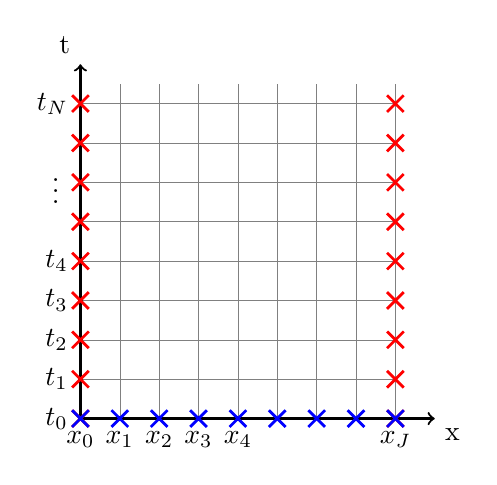
\begin{tikzpicture}[domain=0:4]
	%Grid
	\draw[step=5mm,very thin,color=gray] (0,0) grid (4,4.25);
	%Axis
	\draw[thick,->] (0,0) -- (4.5,0) node[below right] {x};
	\draw[thick,->] (0,0) -- (0,4.5) node[above left] {t};
	\foreach \x in {0,1,2,3,4}
	\draw (5*\x mm,1pt) -- (5*\x mm,-1pt) node[below] {$x_\x$};
	\node[below] at (3,-4pt){$\hdots$};
	\node[below] at (4,-1pt){$x_J$};
	\foreach \y in {0,1,2,3,4}
	\draw (1pt,5*\y mm) -- (-1pt,5*\y mm) node[left] {$t_\y$};
	\node[left] at (-4pt,3){$\vdots$};
	\node[left] at (-1pt,4){$t_N$};
	%Data
	\foreach \x in {0,...,8}{
		\draw[rotate around={45:(0,5*\x mm)},red, line width=1pt] (0.15,5*\x mm) -- (-0.15,5*\x mm);
		\draw[rotate around={135:(0,5*\x mm)},red, line width=1pt] (0.15,5*\x mm) -- (-0.15,5*\x mm);
	}
	\foreach \x in {0,...,8}{
		\draw[rotate around={45:(4,5*\x mm)},red, line width=1pt] (4.15,5*\x mm) -- (3.85,5*\x mm);
		\draw[rotate around={135:(4,5*\x mm)},red, line width=1pt] (4.15,5*\x mm) -- (3.85,5*\x mm);
	}
	\foreach \y in {0,...,8}{
		\draw[rotate around={45:(5*\y mm,0)},blue, line width=1pt] (5*\y mm,0.15) -- (5*\y mm,-0.15);
		\draw[rotate around={135:(5*\y mm,0)},blue, line width=1pt] (5*\y mm,0.15) -- (5*\y mm,-0.15);
	}
	\end{tikzpicture}
	\caption{Datos iniciales y de contorno}
	\label{fig:calor_1}
\end{figure}

Antes de estudiar el método, vamos a definir qué notación se va a utilizar durante toda la descripción del mismo. 
\begin{mdframed}
	\textbf{Notación:}
	\begin{itemize}
		\vspace{-3mm}
	\item $U_j^n$ representa el valor \textbf{obtenido por el método} de la función $u$ evaluada en $x_j,t_n$.
	\item $u_j^n$ representa el valor \textbf{real} de la función $u$ evaluada en $x_j,t_n$.
	\end{itemize}
	Esta notación va a utilizarse de aquí en adelante en todo lo que sigue.
\end{mdframed}

Empezemos recordando que las condiciones de contorno eran las siguientes:
$$u(0,t) = u(1,t) = 0$$
lo que implica que nuestro método ha de cumplir
\begin{equation*}
	\left\{
	\begin{array}{l}
	U_0^n = u_0^n = 0, n\ge 0\\
	U_J^n = u_J^n = 0, n\ge 0
	\end{array}
	\right.
\end{equation*}

Supongamos que $u(x)$ es una solución del problema de la ecuación del calor con los datos iniciales y las condiciones de contorno porporcionados. Podemos aproximar las derivadas $u_{xx}$ y $u_t$ de la siguiente forma:
\begin{align*}
		u_{xx}(x_j, t_n) &\approx \frac{u(x_{j+1}) - 2u(x_j, t_n) + u(x_{j-1}, t_n)}{(\Delta x)^2}\\
		u_t(x_j, t_n) &\approx \frac{u(x_j, t_{n+1})-u(x_j,t_n)}{\Delta t}
\end{align*}

Tenemos un valor aproximado para $u_{xx}$ y $u_t$, luego sabiendo que la ecuación del calor es $u_t = u_{xx}$, podemos construir el siguiente método:
\begin{equation*}
	\frac{U_j^{n+1}-U_j^n}{\Delta t} =  \frac{U_{j+1}^n-2U_j^n+U_{j-1}^n}{(\Delta x)^2}
\end{equation*}
para $n\ge  0$ y $j=1,\hdots ,J-1$.

A partir de aquí, se puede observar que en el método anterior se puede despejar el término que da el valor aproximado de la función en el punto $j$ y en tiempo $n+1$, obteniendo el método explícito:

\begin{mdframed}
	\textbf{Método explícito}
	$$U_j^{n+1} = U_j^n+\nu\left(U_{j+1}^n - 2 U_j^n + U_{j-1}^n\right)$$
	donde $\nu = \frac{\Delta t}{(\Delta x )^2}$
\end{mdframed}

En lo que sigue, utilizando el desarrollo de la serie Taylor, se va a estudiar qué orden tiene esta aproximación.

\subparagraph{Orden del método explícito} 
\mbox{}

Vamos a hallar el desarrollo de Taylor alrededor del punto $x_j, t_n$ del término temporal del método. Vemos que:
$$u(x_j, t_{n+1}) = u(x_j, t_n) + u_t(x_j, t_n)\Delta t +\frac{u_{tt} (x_j,t_n)}{2}\Delta t ^2 + O\left((\Delta t)^3\right)$$

luego:
$$\frac{u(x_j,t_{n+1}) - u(x_j, t_n)}{\Delta t} = u_t(x_j,t_n) + \underbrace{\frac{\Delta t}{2} u_{tt}(x_j,t_n) + O\left((\Delta t)^2\right)}_{\text{error}}$$

Ahora vamos a repetir lo anterior, pero esta vez desarrollaremos la serie de Taylor alrededor del punto $x_j, t_n$ del término espacial del método. 

Tenemos que:
\begin{align*}
u(x_{j+1}, t_n) &= u(x_j,t_n) + u_x(x_j,t_n)\Delta x + u_{xx}(x_j,t_n)\frac{\Delta x^2}{2}\\ &+\  u_{xxx}(x_j,t_n)\frac{\Delta x^3}{3!}  + \hdots\\
\end{align*}

y por otro lado
\begin{align*}
u(x_{j-1},t_n) &= u(x_j, t_n) - u_x(x_j,t_n)\Delta x + u_{xx}(x_j,t_n)\frac{(\Delta x)^2}{2}\\ &-\ u_{xxx}(x_j, t_n)\frac{(\Delta x)^3}{3!} + u_{xxxx}(x_j,t_n)\frac{(\Delta x)^4}{4!} + \hdots
\end{align*}

finalmente obtenemos:
$$\frac{u(x_{j+1}, t_n) - 2u(x_j,t_n) + u(x_{j-1},t_n)}{(\Delta x)^2} = u_{xx}(x_j,t_n) + \underbrace{ u_{xxxx}(x_j, t_n)\frac{\Delta x^2}{12} + O\left((\Delta x)^4\right)}_{\text{error}}$$

Como conclusión tenemos que el método explícito utiliza una diferencia finita de primer orden para aproximar la derivada temporal y una diferencia finita de segundo orden para aproximar la derivada espacial.

\subparagraph{Error de truncación}\mbox{}

\begin{defn}[Error de truncacion]
Se llama error de truncación del método numérico al residuo que se obtiene cuando se aplica el método a la solución exacta.
\end{defn}

El error de truncación del método explícito, atendiendo a la definición anterior, tiene la expresión:
$$T(x_j,t_n) = \frac{u(x_j,t_{n+1})-u(x_j,t_n)}{\Delta t} - \frac{u(x_{j+1},t_n)-2u(x_j,t_n)+u(x_{j-1},t_n)}{\Delta x^2}$$

Supongamos que $u(x,t)$ es la solución exacta del problema de la ecuación del calor. Vamos a hallar, mediante el desarrollo de Taylor, el error de truncación del método explícito:
\begin{align*}
T(x_j,t_n) &= \frac{u(x_j,t_{n+1})-u(x_j,t_n)}{\Delta t} - \frac{u(x_{j+1},t_n)-2u(x_j,t_n)+u(x_{j-1},t_n)}{\Delta x^2}\\ 
& =  u_t(x_j,t_n) + u_{tt}(x_j,t_n)\frac{\Delta t}{2} + O \left((\Delta t)^2\right) \\
& - u_{xx}(x_j,t_n) + u_{xxxx}(x_j,t_n)\frac{\Delta x^2}{12} + O\left((\Delta x)^4\right)\\ 
& =  u_{tt}(x_j,t_n)\frac{\Delta t}{2} -  u_{xxxx}(x_j,t_n)\frac{\Delta x^2}{12} + O\left((\Delta t)^2\right) + O\left((\Delta x)^4\right)
\end{align*}

En el último paso, se ha tenido en cuenta que $u_t = u_{xx}$. Otra forma escribir el error de truncación es la que sigue:
$$T_j^n = \Delta t \left(\frac{u_{tt}(x_j,t_n)}{2}- \frac{1}{12\nu} u_{xxxx}(x_j,t_n)\right) + O\left((\Delta t)^2\right) + O\left((\Delta x)^4\right)$$

Si tomamos $\xi_n \in (t_n,t_{n+1})$ y $\eta_j \in (x_{j-1}, x_{j+1})$ podemos eliminar los términos para la comparación asintótica:
$$T_j^n = \Delta t \left(\frac{u_{tt}(x_j,\xi_n)}{2}- \frac{1}{12\nu} u_{xxxx}(\eta_j,t_n)\right)$$

\subparagraph{Cota para el error de truncación}\mbox{}

Si tomamos $M_{tt}$ y $M_{xxxx}$ como cota para $u_{tt}$ y $u_{xxxx}$, tenemos el error de truncación acotado como sigue:

$$|T_j^n| \le \Delta t \left(\frac{M_{tt}}{2} + \frac{M_{xxxx}}{12{\nu}}\right)$$

Dado que la ecuación del calor establece que $u_{t} = u_{xx}$, entonces, asumiendo regularidad en la solución, se tiene que $(u_t)_{t} = (u_{t})_{xx} = u_{xxxx}$. 

Como caso particular, si tomamos $\nu = 1/6$ se cumple :
$$T_j^n = \Delta t\cdot 0 + O\left((\Delta t)^2\right) + O\left((\Delta x)^4\right) = O\left((\Delta t)^2\right)$$
obteniendo así orden 2 para el error de truncación.

\subparagraph{Convergencia del método}\mbox{}

El método explícito es consistente porque el error de truncación tiende a cero cuando $\Delta t \to 0$.
Además es incondicionalmente consistente, lo que quiere decir que $T_j^n$ tiende hacia cero independientemente de los valores de $\Delta t$ y $\Delta x$ (más concretamente de su relación $\nu = \frac{\Delta t}{(\Delta x)^2}$).

En esta sección se va a estudiar la convergencia del método, antes de ello, vamos a ver qué necesitamos para demostrar que es convergente.

\begin{prop}
	$$\text{Estabilidad} + \text{Consistencia} \iff \text{Convergencia}$$
\end{prop} 

A partir de esta proposición y dado que el método es incondicionalmente consistente, basta que sea estable para que sea convergente.

\begin{prop}
$$\text{El método es estable} \iff \nu \le \frac{1}{2}$$
\end{prop}

\begin{proof}
	
Vamos a ver, utilizando el principio del máximo, que si $\nu < \frac{1}{2}$, el método es estable. Tenemos que:
\begin{align*}
u_j^{n+1} &= u_j^n + \nu (u_{j+1}^n-2u_j^n+u_{j-1}^n) + T_j^n \Delta t\\
U_j^{n+1} &= U_j^n + \nu (U_{j+1}^n-2U_j^n+U_{j-1}^n)
\end{align*}

Denotamos con $e_j^n$ al residuo del método, de forma que:
$$e_j^n = U_j^n - u_j^n$$

Calculamos el error de paso:
$$e_j^{n+1} = e_j^n + \nu (e_{j+1}^n-2e_j^n+e_{j-1}^n) - T_j^n \Delta t$$

Operando y suponiendo que $\nu \le \frac{1}{2}$ queda:
$$e_j^{n+1} = \nu e_{j+1}^n + \underbrace{(1-2\nu)}_{\ge 0} e_j^n + \nu e_{j-1}^n - T_j^n \Delta t$$

Ahora definimos
$$E^n = \max_{0\le j \le J} |e_j^n|$$

y acotamos el error:
\begin{equation*}
	\begin{array}{lll}
	|e_j^{n+1}| &\le& \nu|e_{j+1}^n| + (1-2\nu) |e_j^n| + \nu |e_{j-1}^n| +  \bar{T}\Delta t\\
	&\le& \nu E^n +(1-2\nu)E^n + \nu E^n + \bar{T}\Delta t\\
	&=& E^n + \bar{T} \Delta t
	\end{array}
\end{equation*}

Donde $$\bar{T} = \Delta t \left( \frac{M_{tt}}{2} + \frac{M_{xxxx}}{12\nu}  \right)$$

es decir, $\bar{T}$ es la cota para el error de truncación. 

\subparagraph*{Conclusión}\mbox{}

Como $E^0 = 0$ y $E^n = (n\bar{T})\Delta t \le t_f \bar{T}$, tenemos que $$E^n \to 0 \text{ cuando }\Delta t \to 0$$ 

es decir, el método es estable.
\end{proof}

Dado que hemos obtenido que el método es estable si $\nu <\frac{1}{2}$ e incondicionalmente consistente, tenemos que bajo la misma condición, el método es convergente.

\newpage

\subparagraph{Programación del método}\mbox{}

Sabemos que inicialmente tenemos los siguientes datos
\begin{equation*}
	\left\{
	\begin{array}{l r}
		u(0,t) = 0\\
		u(1,t) = 0\\
		u(x,0) = u_0(x)
	\end{array}
	\right.
\end{equation*}

Es decir, que disponemos de los datos iniciales (en tiempo $t=0$) y de contorno (cuando $x=0$ y $x=1$). Partiendo de ellos podemos calcular el resto de datos como ya hemos visto:

$$U_j^{n+1} = U_j^n+\nu\left(U_{j+1}^n - 2 U_j^n + U_{j-1}^n\right)$$

El algoritmo vectorial tendría la siguiente forma:
\begin{equation*}
	\begin{array}{l l l}
		\begin{bmatrix}
			U_1^{n+1}\\
			U_2^{n+1}\\
			\vdots\\
			U_{J-1}^{n+1}\\
		\end{bmatrix}
		=
		\begin{bmatrix}
			1-2\nu & \nu       &        & \\
			\nu    & \ddots    & \ddots & \\
			          & \ddots & \ddots & \nu\\
			          &        & \nu    & 1-2\nu\\
		\end{bmatrix}
		\begin{bmatrix}
			U_1^{n}\\
			U_2^{n}\\
			\vdots\\
			U_{J-1}^{n}\\
		\end{bmatrix}
	\end{array}
\end{equation*}

Gráficamente, lo que estamos realizando es obtener una aproximación (utilizando la aproximación de las derivadas) del siguiente punto de la partición en la derivada temporal a partir tres puntos en la derivada espacial (ver figura \ref{fig:calor_2}). De esta forma, sólo usando los datos iniciales y de contorno obtenemos un valor para cada uno de los puntos del mallado.

\begin{figure}[h]
	\centering
	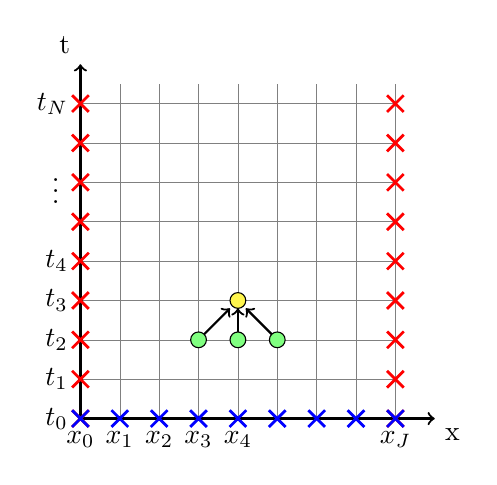
\begin{tikzpicture}[domain=0:4]
	%Grid
	\draw[step=5mm,very thin,color=gray] (0,0) grid (4,4.25);
	%Axis
	\draw[thick,->] (0,0) -- (4.5,0) node[below right] {x};
	\draw[thick,->] (0,0) -- (0,4.5) node[above left] {t};
	\foreach \x in {0,1,2,3,4}
	\draw (5*\x mm,1pt) -- (5*\x mm,-1pt) node[below] {$x_\x$};
	\node[below] at (3,-4pt){$\hdots$};
	\node[below] at (4,-1pt){$x_J$};
	\foreach \y in {0,1,2,3,4}
	\draw (1pt,5*\y mm) -- (-1pt,5*\y mm) node[left] {$t_\y$};
	\node[left] at (-4pt,3){$\vdots$};
	\node[left] at (-1pt,4){$t_N$};
	%Data
	\foreach \x in {0,...,8}{
		\draw[rotate around={45:(0,5*\x mm)},red, line width=1pt] (0.15,5*\x mm) -- (-0.15,5*\x mm);
		\draw[rotate around={135:(0,5*\x mm)},red, line width=1pt] (0.15,5*\x mm) -- (-0.15,5*\x mm);
	}
	\foreach \x in {0,...,8}{
		\draw[rotate around={45:(4,5*\x mm)},red, line width=1pt] (4.15,5*\x mm) -- (3.85,5*\x mm);
		\draw[rotate around={135:(4,5*\x mm)},red, line width=1pt] (4.15,5*\x mm) -- (3.85,5*\x mm);
	}
	\foreach \y in {0,...,8}{
		\draw[rotate around={45:(5*\y mm,0)},blue, line width=1pt] (5*\y mm,0.15) -- (5*\y mm,-0.15);
		\draw[rotate around={135:(5*\y mm,0)},blue, line width=1pt] (5*\y mm,0.15) -- (5*\y mm,-0.15);
	}
		\draw[thick,->] (1.5,1) -- (1.9,1.4);
		\draw[thick,->] (2,1) -- (2,1.4);
		\draw[thick,->] (2.5,1) -- (2.1,1.4);
	\draw[fill=green!50!white, draw=black] (1.5,1) circle (1mm);
	\draw[fill=green!50!white, draw=black] (2,1) circle (1mm);
	\draw[fill=green!50!white, draw=black] (2.5,1) circle (1mm);
	\draw[fill=yellow!70!white, draw=black] (2,1.5) circle (1mm);
	\end{tikzpicture}
	\caption{Método en diferencias finitas: $U_j^{n+1} = U_j^n+\nu\left(U_{j+1}^n - 2 U_j^n + U_{j-1}^n\right)$}
	\label{fig:calor_2}
\end{figure}

\newpage
\subparagraph{Análisis de Fourier del método explícito}\mbox{}

Hemos visto que la solución general para el problema de la ecuación del calor tiene la siguiente forma:
$$u(x, t) = \sum_{m=1}^\infty B_m e^{-(m\pi)^2 t} sin(m\pi x)$$

Equivalentemente, podemos reescribir lo anterior del siguiente modo:
$$u(x,t) = \sum_{m=-\infty}^\infty B_m e^{-(m\pi)^2 t}e^{i(m\pi)x}$$

Para la solución teórica, los modos de Fourier $e^{-k^2t}$ y $e^{ikx}$ definiendo \framebox{$k=m\pi$} y \framebox{$m=-\infty,\hdots, \infty$}, son soluciones particulares.

Para realizar el análisis de Fourier del método explícito vamos a definir un factor $\lambda(k)$ al que llamaremos factor de amplifiación:
$$\lambda(k) \simeq e^{-k^2\Delta t}$$ 

Ahora buscamos $U_j^n$ de la forma
\begin{equation*}
	\begin{array}{l l l}
		U_j^n =\lambda^n e^{ik(j\Delta x)}&\simeq& \left[e^{-k^2\Delta t}\right]^n\ e^{ik(j\Delta x)}\\
				&=& e^{-k^2n\Delta t}\ e^{ik(j\Delta x)}\\
				&=& e^{-k^2t_n}\ e^{ikx_j}\\
	\end{array}
\end{equation*}

Sustituyendo en el método explícito tenemos que
$$\lambda^{n+1}e^{ik(j\Delta x)} =
\lambda^ne^{ik(j\Delta x)} + \nu\left[\lambda^n e^{ik(j+1)\Delta x}-2\lambda^n e^{ik(j\Delta x)}+\lambda^n e^{ik(j-1)\Delta x}\right]$$

Dividiendo por $\lambda^n e^{ik(j\Delta x)}$
\begin{equation*}
	\begin{array}{l l l}
		\lambda(k) & = & 1+\nu\left[e^{ik\Delta x} -2 + e^{-ik\Delta x}\right]\\
		& = & 1 + \nu \left[2cos(k\Delta x)-2\right]\\
		& = & 1 + \nu \left[2\left(1-2sin^2(\frac{k}{2}\Delta x)\right)-2\right]\\
		& = & 1 + \nu \left[-4sin^2(\frac{k}{2}\Delta x)\right]\\
	\end{array}
\end{equation*}

Tomando $U_j^n = \lambda(k)^n e^{ikj\Delta x}$ se verifica el método y como aproximación tomamos
$$U_j^n = \sum_{m=-\infty}^\infty B_m \lambda(k)^n e^{ikj\Delta x}$$

\subparagraph*{Comportamiento cualitativo de $\lambda(k)$.}\mbox{}

El método presenta insestabilidad si $|\lambda(k)| > 1$ dado que $$|\lambda(k)| > 1 \implies |\lambda(k)|^n \to \infty$$ 

Tenemos estabilidad si y sólo si $|\lambda(k)| \le 1$. Esto es equivalente a decir que podemos acotar dos aproximaciones numéricas del método en términos de los datos iniciales. Supongamos dos datos iniciales para $t=0$:
\begin{equation*}
	\left\{
	\begin{array}{l}
		u_0^{(1)}(x) = \sum_{m=1}^\infty B_m^1 e^{ikx}\\
		u_0^{(2)}(x) = \sum_{m=1}^\infty B_m^2 e^{ikx}
	\end{array}
	\right.
\end{equation*}

Obtenemos las aproximaciones de la solución los problemas partiendo de dichos datos:
\begin{equation*}
\left\{
\begin{array}{l}
	(U_j^n)^{(1)} = \sum_{m=-\infty}^\infty B_m^1 \lambda(k)^n e^{ik(j\Delta x)}\\
	(U_j^n)^{(2)} = \sum_{m=-\infty}^\infty B_m^2 \lambda(k)^n e^{ik(j\Delta x)}\\
\end{array}
\right.
\end{equation*}

La diferencia entre las dos aproximaciones es
$$(U_j^n)^{(1)} - (U_j^n)^{(2)} = \sum_{m=-\infty}^\infty (B_m^1-B_m^2) \lambda(k)^n e^{ik(j\Delta x)}$$

Tomando normas
$$\left|(U_j^n)^{(1)}-(U_j^n)^{(2)}\right| \le \left|\sum_{m=-\infty}^\infty (B_m^1-B_m^2) e^{ik(j\Delta x)}\right| = \left|u_0^{(1)}(x_j)-u_0^{(2)}(x_j)\right|$$

\subparagraph*{Comportamiento cuantitativo de $\lambda(k)$.}\mbox{}

Vamos a comparar $e^{-k^2\Delta t}$ y $\lambda(k)$. Para ello, desarrollamos las series de Taylor de ambos términos:

\begin{align*}
		e^{-k^2\Delta t} & =  1-k^2\Delta t + \frac{1}{2}k^4\Delta t ^2 + O(\Delta t ^3)\\
		\lambda(k) & =  1-4\nu sin^2(\frac{k}{2}\Delta x)\\
		& =  1-4\nu\left[\frac{k^2}{4}\Delta x^2 - \frac{1}{3}\frac{k^4}{16}\Delta x^4 + \hdots \right]\\
		& =  1-k^2\Delta t + \frac{k^4}{12}\Delta t \Delta x^2 + \hdots
\end{align*}

Obteniendo la diferencia
$$\lambda(k) - e^{-k^2\Delta t} = \frac{k^4\Delta t \Delta x^2}{12} - \frac{k^4\Delta t^2}{2} + O(\Delta t ^3)$$

En general
$\lambda(k) - e^{-k^2\Delta t} = O(\Delta t^2)$, es decir, que el método tiene orden 1 de consistencia.

Se puede ver mejor si lo reescribimos de la forma:
$$\lambda(k) - e^{-k^2\Delta t} = \left[\frac{k^4}{12\nu}-\frac{k^4}{2}\right]\Delta t^2 + O(\Delta t^3)$$

Vemos de nuevo que si $\nu = \frac{1}{6}$ se tiene orden 2 de consistencia.

\subparagraph*{Convergencia del método explícito} \mbox{}

Ya sabemos que 
$$\lambda(k) = 1-4\nu sin^2(\frac{k}{2}\Delta x)$$ 

y que tenemos estabilidad si y sólo si \framebox{$|\lambda(k)|\le 1$}. 

Analizando $\lambda(k)$ vemos que
$$|\lambda(k)| = \left|1-4\nu sin^2\left(\frac{k}{2}\Delta x\right)\right|\le \left|1-4\nu\right|$$

Vamos a distinguir dos casos
\begin{itemize}
	\item Si $1-4\nu\ge 0 \implies 1-4\nu \le 1$
	\item Si $1-4\nu < 0\implies |1-4\nu| = -1+4\nu < 1 \iff 4\nu \le 2 \iff \nu \le \frac{1}{2}$ 
\end{itemize}

En el caso inestable ($\nu > \frac{1}{2}$) la frecuencia más inestable es $k = J\pi$, donde se obtienen oscilaciones:
$$\lambda^n e^{ikj\Delta x} = \lambda^n e^{iJ\pi j\frac{1}{J}} = \lambda^n e^{i\pi j} = \lambda^n cos(\pi j)$$

Veamos otra forma para ver que el método converge utilizando análisis de Fourier.

Por un lado tenemos la solución del problema
\begin{equation*}
		u(x,t)  =  \sum_{m=-\infty}^{\infty} B_m e^{(-m\pi)^2t}e^{im\pi x}
\end{equation*}

Y por otro el dato inicial
\begin{equation*}
	u(x,t)  =  \sum_{m=-\infty}^{\infty} B_m e^{im\pi x}
\end{equation*}

En el método explícito teníamos
\begin{equation*}
	U_j^n  =  \sum_{m=-\infty}^{\infty} \lambda^n(k)B_m e^{ik j\Delta x}
\end{equation*}

Hallamos $e_j^n$:
\begin{equation*}
	e_j^n = U_j^n - u_j^n =  \sum_{m=-\infty}^{\infty} B_m e^{ik j\Delta x}\left(\lambda^n(k) - e^{-k^2n\Delta t}\right)
\end{equation*}

Vamos a probar que $\forall \varepsilon > 0$ $\exists \Delta t_0$ tal que si $\Delta t \le \Delta t_0 \implies |e_j^n| < \varepsilon$ con la condición impuesta de que $\nu\le\frac{1}{2}$.

Como hipótesis de regularidad asumimos que la serie de Fourier de $u(x)$ es absolutamente convergente en $[0,1]$.

Fijamos $\nu$ y $\varepsilon > 0$. Existe un $m_0$ tal que $$\sum_{|m|>m_0} |B_m|\le \frac{1}{4}\varepsilon$$

Vamos a analizar $|e_j^n|$ en dos partes:
\begin{equation*}
	|e_j^n| \le \underbrace{\sum_{|m|>m_0}|B_m|\left(|\lambda^n(k)|+\left|e^{-k^2n\Delta t}\right|\right)}_1 + \underbrace{\sum_{|m|\le m_0}|B_m|\left|\lambda^n(k)-e^{-k^2n\Delta t}\right|}_2
\end{equation*}

Antes de comenzar el análisis es necesario enunciar el siguiente lema.
\begin{lemma}
	$$|\lambda| \le 1\text{ y }|\nu|\le 1 \implies |\lambda^n-\nu^n|\le n|\lambda-\nu|$$
\end{lemma}

La demostración de este lema se realiza por inducción. Ahora estudiamos los dos términos de la expresión para $|e_j^n|$:

\begin{enumerate}
	\item Utilizando que $|\lambda(k)| \le 1$ se acota $(1)$ por $$\sum_{|m|>m_0}2|B_m|$$
	\item Usando el lema llegamos a que
	$$\sum_{|m|\le m_0}{|B_m|\cdot n\cdot \left|\lambda(k)-e^{-k^2\Delta t}\right|} \le \sum_{|m|\le m_0}{|B_m|\cdot n \cdot C(\nu)k^4(\Delta t)^2}$$
	
	Sabiendo que $n\Delta t\le t_f$
	$$\sum_{|m|\le m_0}{|B_m|\cdot n \cdot C(\nu)k^4(\Delta t)^2} \le \left[\sum_{|m|\le m_0}|B_m|t_fC(\nu)k^4\right]\Delta t$$
	
	Si tomamos $\Delta t\le \frac{\varepsilon}{2}\frac{1}{C}\le\frac{\varepsilon}{2}$ llegamos a que
	$$|e_j^n| \le \frac{\varepsilon}{2} + \frac{\varepsilon}{2} = \varepsilon$$
\end{enumerate}

\subparagraph{Efecto computacional}\mbox{}

De las infinitas frecuencias $m=-\infty\hdots\infty$ sólo hay un número finito de frecuencias distintas a efectos del odenador. Tenemos que para la función $e^{im\pi x}$ evaluada en una malla, el ordenador ve los valores en $J+1$ puntos desde $j=0$ hasta $j = J$. 

Si $m_1\pi = m_2\pi + 2lJ$ con $l=\pm1,\pm2,\hdots$, entonces $e^{im_1\pi x}$ y $e^{im_2\pi x}$ son indistinguibles en la malla (ver figura \ref{fig:frecmalla}).
En la práctica sólo tenemos frecuencias distintas para $$j=-(J-1), -(J-2), \hdots, 0, 1, \hdots, J$$

Las frecuencias se llaman alias, y el error se llama error de aliasis.
\begin{equation*}
	e^{im_1\pi j\Delta x} = e^{im_1\pi j / J} = e^{im_2\pi j / J}\underbrace{e^{i2l\pi j}}_{=1}
\end{equation*}

\begin{figure}[h]
	\centering
	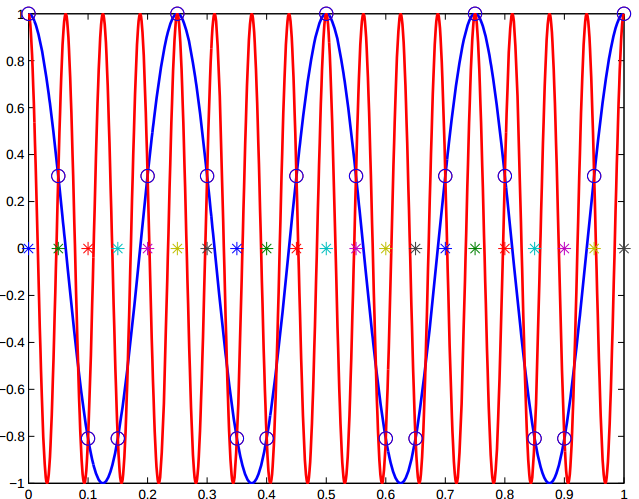
\includegraphics[width=\textwidth/2]{img/frecmalla.png}
	\caption{En la figura se pueden observar que para dos frecuencias distintas, en los puntos de la malla ambas tienen el mismo valor, por tanto son indistinguibles para el ordenador.}
	\label{fig:frecmalla}
\end{figure}

 \begin{example}
 	$$U_j^n = \sum_{m=-\infty}^\infty B_m\lambda(m\pi)e^{im\pi x}$$
	Vamos a tomar una malla $J=20$, es decir, tenemos $21$ puntos en $[0,1]$.
	Elegimos por ejemplo $m=8$. En la figura \ref{fig:frecmalla} se puede observar
	\begin{itemize}
		\item En azul $cos(8\pi x)$.
		\item En rojo $cos(-32\pi x)$.
	\end{itemize}
	En todos los puntos de la malla, las funciones coinciden.
 \end{example}
 
\paragraph{Método implícito}\mbox{}

En el método explícito tenemos la restricción $\nu=\frac{\Delta t}{\Delta x ^2} \le \frac{1}{2}$, es decir, $\Delta t \le \frac{\Delta x ^2}{2}$. En la práctica, a medida que se refina la malla para la variable $x$, se tiene que aumentar muchísimo el número de pasos en tiempo para llegar al tiempo final.
 
Vamos a construir un método implícito mediante la siguiente expresión:
$$\frac{U_j^{n+1}-U_j^n}{\Delta t} = \frac{U_{j+1}^{n+1}-2U_{j}^{n+1}+U_{j-1}^{n+1}}{\Delta x^2}$$

Obteniendo:
$$U_j^{n+1} = U_j^n + \nu \left[U_{j+1}^{n+1}-2U_{j}^{n+1}+U_{j-1}^{n+1}\right]$$

\subparagraph{Programación del método}\mbox{}

Matricialmente, el método tiene la siguiente expresión:
\begin{equation*}
		\begin{array}{l l l}
			\begin{bmatrix}
				U_1^{n}\\
				U_2^{n}\\
				\vdots\\
				U_{J-1}^{n}\\
			\end{bmatrix}
			=
			\underbrace{
			\begin{bmatrix}
				1+2\nu & -\nu       &        & \\
				-\nu    & \ddots    & \ddots & \\
				& \ddots & \ddots & -\nu\\
				&        & -\nu    & 1+2\nu\\
			\end{bmatrix}}_{A}
			\begin{bmatrix}
				U_1^{n+1}\\
				U_2^{n+1}\\
				\vdots\\
				U_{J-1}^{n+1}\\
			\end{bmatrix}
		\end{array}
\end{equation*}

En la figura \ref{fig:calor_impl} se puede observar cómo obtiene el método los valores de un punto a partir del resto.

\begin{figure}[h]
	\centering
	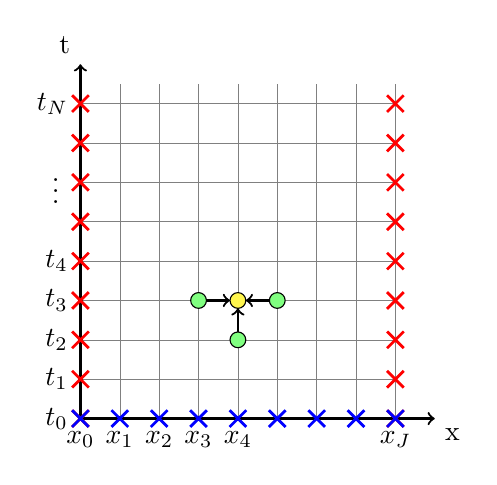
\begin{tikzpicture}[domain=0:4]
	%Grid
	\draw[step=5mm,very thin,color=gray] (0,0) grid (4,4.25);
	%Axis
	\draw[thick,->] (0,0) -- (4.5,0) node[below right] {x};
	\draw[thick,->] (0,0) -- (0,4.5) node[above left] {t};
	\foreach \x in {0,1,2,3,4}
	\draw (5*\x mm,1pt) -- (5*\x mm,-1pt) node[below] {$x_\x$};
	\node[below] at (3,-4pt){$\hdots$};
	\node[below] at (4,-1pt){$x_J$};
	\foreach \y in {0,1,2,3,4}
	\draw (1pt,5*\y mm) -- (-1pt,5*\y mm) node[left] {$t_\y$};
	\node[left] at (-4pt,3){$\vdots$};
	\node[left] at (-1pt,4){$t_N$};
	%Data
	\foreach \x in {0,...,8}{
		\draw[rotate around={45:(0,5*\x mm)},red, line width=1pt] (0.15,5*\x mm) -- (-0.15,5*\x mm);
		\draw[rotate around={135:(0,5*\x mm)},red, line width=1pt] (0.15,5*\x mm) -- (-0.15,5*\x mm);
	}
	\foreach \x in {0,...,8}{
		\draw[rotate around={45:(4,5*\x mm)},red, line width=1pt] (4.15,5*\x mm) -- (3.85,5*\x mm);
		\draw[rotate around={135:(4,5*\x mm)},red, line width=1pt] (4.15,5*\x mm) -- (3.85,5*\x mm);
	}
	\foreach \y in {0,...,8}{
		\draw[rotate around={45:(5*\y mm,0)},blue, line width=1pt] (5*\y mm,0.15) -- (5*\y mm,-0.15);
		\draw[rotate around={135:(5*\y mm,0)},blue, line width=1pt] (5*\y mm,0.15) -- (5*\y mm,-0.15);
	}
	\draw[thick,->] (1.5,1.5) -- (1.9,1.5);
	\draw[thick,->] (2,1) -- (2,1.4);
	\draw[thick,->] (2.5,1.5) -- (2.1,1.5);
	\draw[fill=green!50!white, draw=black] (1.5,1.5) circle (1mm);
	\draw[fill=green!50!white, draw=black] (2,1) circle (1mm);
	\draw[fill=green!50!white, draw=black] (2.5,1.5) circle (1mm);
	\draw[fill=yellow!70!white, draw=black] (2,1.5) circle (1mm);
	\end{tikzpicture}
	\caption{Método implícito: $U_j^{n+1} = U_j^n + \nu \left[U_{j+1}^{n+1}-2U_{j}^{n+1}+U_{j-1}^{n+1}\right]$}
	\label{fig:calor_impl}
\end{figure}

Hay que resolver el sistema lineal de la matriz $A$, para cada paso en el tiempo se resuelve el sistema de la matriz tridiagonal, que es diagonalmente dominante, es decir:
$$|1+2\nu|\ge |-\nu|+|-\nu|$$

En \textsc{MatLab}, para introducir $A$, introducimos sólo los 3 vectores de las diagonales y resolvemos el sistema por eliminación gaussiana, sin ser necesario utilizar pivotaje.
\begin{lstlisting}
	% Para resolver un sistema lineal Ax = B usamos
	x = A\B;
\end{lstlisting}

Dado que la matrix $A$ tiene dimensión $(n-1)\times(n-1)$, el coste computacional de resolver el sistema es $O(3*(J-1))$.

\newpage
Veamos un ejemplo de como construir una matriz tridiagonal en \textsc{MatLab}.
\begin{lstlisting}
	% Elegimos el valor para J y para nu.
	J = 20;
	nu = 0.4;
	
	% Creamos un vector columna de J-1 elementos con todos 
	% los valores a 1 (diagonal).
	e = ones(J - 1, 1);
	e = (1 + 2*nu) * e;
	
	% Creamos un vector columna de J-2 elementos con todos
	% los valores a 1 (diagonal superior)
	eu = ones(J - 2, 1);
	eu = -nu * eu;
	
	% Creamos un vector columna de J-2 elementos con todos 
	% los valores a 1 (diagonal inferior)
	ed = eu;
	
	% Agregamos un cero al principio de la diagonal superior
	% (para que tenga J-1 elementos)
	eu = [0, eu];
	
	% Agregamos un cero al final de la diagonal inferior
	% (para que tenga J-1 elementos)
	ed = [ed, 0];
	
	% Creamos la matriz tridiagonal
	A = spdiags([ed e eu], -1:1, J-1, J-1);
\end{lstlisting}  

\subparagraph{Análisis de Fourier del método implícito}\mbox{}

El método implícito, como ya hemos visto, tiene la expresión:
$$U_j^{n+1} = U_j^n + \nu \left[U_{j+1}^{n+1}-2U_{j}^{n+1}+U_{j-1}^{n+1}\right]$$

Buscamos $U_j^n$ de la forma:
$$U_j^n = \lambda^n e^{ik j\Delta x}$$

Sustituyendo en el método, obtenemos:
$$\lambda^{n+1} e^{ik j\Delta x} = \lambda^n e^{ik j\Delta x} + \nu \left[\lambda^{n+1}e^{ik ({j+1})\Delta x} - 2\lambda^{n+1}e^{ik j\Delta x}+\lambda^{n+1}e^{ik ({j-1})\Delta x}\right]$$

Dividiendo por $\lambda^n e^{ik j\Delta x}$ obtenemos la siguiente expresión para $\lambda(k)$:
\begin{align*}
	\lambda(k) & = 1+\nu\left[\lambda e^{ik\Delta x}-2\lambda + \lambda e^{-ik\Delta x}\right]\\
	& =  1+\lambda \nu\left[e^{ik\Delta x} - 2 + e^{-ik\Delta x}\right]\\
	& = 1-4\nu\lambda sin^2\left(\frac{k}{2}\Delta x\right)\\
\end{align*}

Resolviendo el sistema:
$$\lambda(k) = \frac{1}{1+4\nu sin^2\left(\frac{k}{2}\Delta x\right)}$$

El método implícito es incondicionalmente estable, lo que quiere decir que es siempre estable independientemente de los valores de $\Delta t$ y $\Delta x$.

\paragraph{El $\theta$-método}\mbox{}

El $\theta$-método es un método que combina el método explícito y el método implícito de la siguiente forma, con $0\le\theta\le 1$:
$$\frac{U_j^{n+1}-U_j^n}{\Delta t} = 
\theta \left[\frac{U_{j+1}^{n+1}-2U_{j}^{n+1}+U_{j-1}^{n+1}}{(\Delta x)^2}\right] +
(1-\theta) \left[ \frac{U_{j+1}^n-2U_j^n+U_{j-1}^n}{(\Delta x)^2}\right]$$

Según el valor de $\theta$ se tiene:
\begin{itemize}
	\vspace{-3mm}
	\item $\theta = 0$ Método explícito (estable si $\nu \le \frac{1}{2}$).
	\item $\theta = 1$ Método implícito siempre de orden 1.
\end{itemize}

Otra forma de escribirlo es
$$U_j^{n+1} = U_j^n + \nu\theta\left[U_{j+1}^{n+1} - 2U_{j}^{n+1} + U_{j-1}^{n+1}\right] + \nu(1-\theta)\left[U_{j+1}^{n}-2U_{j}^{n}+U_{j-1}^{n}\right]$$

\subparagraph{Programación del método}\mbox{}

Matricialmente, el método tiene la expresión:
\begin{equation*}
	\begin{array}{l l l}
		\underbrace{
		\begin{bmatrix}
			1+2\nu\theta & -\nu\theta &        & \\
			-\nu\theta   & \ddots     & \ddots & \\
			& \ddots     & \ddots     & -\nu\theta\\
			&            & -\nu\theta & 1+2\nu\theta\\
		\end{bmatrix}}_A
		\begin{bmatrix}
			U_1^{n+1}\\
			U_2^{n+1}\\
			\vdots\\
			U_{J-1}^{n+1}\\
		\end{bmatrix}
		=\\
		\underbrace{
		\begin{bmatrix}
			1-(1-\theta)2\nu         & (1-\theta)\nu&        & \\
			(1-\theta)\nu            & \ddots       & \ddots & \\
			& \ddots & \ddots        & (1-\theta)\nu\\
			&        & (1-\theta)\nu & 1-(1-\theta)2\nu\\
		\end{bmatrix}}_B
			\begin{bmatrix}
				U_1^{n}\\
				U_2^{n}\\
				\vdots\\
				U_{J-1}^{n}\\
			\end{bmatrix}
	\end{array}
	\end{equation*}
	
	Hay que resolver el sistema lineal en el que $A$ y $B$ son matrices tridiagonales y diagonalmente dominantes:
	$$|1+2\nu\theta| > |-\nu\theta| + |-\nu\theta|$$
	
	En la figura \ref{fig:calor_theta} se puede observar cómo obtiene el método los valores de un punto a partir del resto.
	
	\begin{figure}[h]
		\centering
		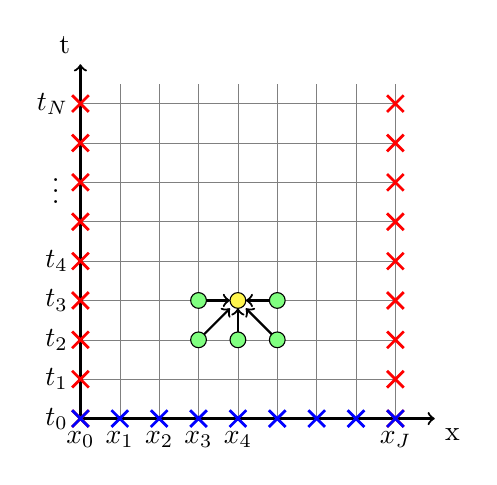
\begin{tikzpicture}[domain=0:4]
		%Grid
		\draw[step=5mm,very thin,color=gray] (0,0) grid (4,4.25);
		%Axis
		\draw[thick,->] (0,0) -- (4.5,0) node[below right] {x};
		\draw[thick,->] (0,0) -- (0,4.5) node[above left] {t};
		\foreach \x in {0,1,2,3,4}
		\draw (5*\x mm,1pt) -- (5*\x mm,-1pt) node[below] {$x_\x$};
		\node[below] at (3,-4pt){$\hdots$};
		\node[below] at (4,-1pt){$x_J$};
		\foreach \y in {0,1,2,3,4}
		\draw (1pt,5*\y mm) -- (-1pt,5*\y mm) node[left] {$t_\y$};
		\node[left] at (-4pt,3){$\vdots$};
		\node[left] at (-1pt,4){$t_N$};
		%Data
		\foreach \x in {0,...,8}{
			\draw[rotate around={45:(0,5*\x mm)},red, line width=1pt] (0.15,5*\x mm) -- (-0.15,5*\x mm);
			\draw[rotate around={135:(0,5*\x mm)},red, line width=1pt] (0.15,5*\x mm) -- (-0.15,5*\x mm);
		}
		\foreach \x in {0,...,8}{
			\draw[rotate around={45:(4,5*\x mm)},red, line width=1pt] (4.15,5*\x mm) -- (3.85,5*\x mm);
			\draw[rotate around={135:(4,5*\x mm)},red, line width=1pt] (4.15,5*\x mm) -- (3.85,5*\x mm);
		}
		\foreach \y in {0,...,8}{
			\draw[rotate around={45:(5*\y mm,0)},blue, line width=1pt] (5*\y mm,0.15) -- (5*\y mm,-0.15);
			\draw[rotate around={135:(5*\y mm,0)},blue, line width=1pt] (5*\y mm,0.15) -- (5*\y mm,-0.15);
		}
		\draw[thick,->] (1.5,1.5) -- (1.9,1.5);
		\draw[thick,->] (2,1) -- (2,1.4);
		\draw[thick,->] (2.5,1.5) -- (2.1,1.5);
		\draw[thick,->] (1.5,1) -- (1.9,1.4);
		\draw[thick,->] (2.5,1) -- (2.1,1.4);
		\draw[fill=green!50!white, draw=black] (1.5,1.5) circle (1mm);
		\draw[fill=green!50!white, draw=black] (2,1) circle (1mm);
		\draw[fill=green!50!white, draw=black] (2.5,1.5) circle (1mm);
		\draw[fill=green!50!white, draw=black] (1.5,1) circle (1mm);
		\draw[fill=green!50!white, draw=black] (2.5,1) circle (1mm);
		\draw[fill=yellow!70!white, draw=black] (2,1.5) circle (1mm);
		\end{tikzpicture}
		\caption{El $\theta$-método}
		\label{fig:calor_theta}
	\end{figure}

\subparagraph{Análisis de Fourier del método}\mbox{}

Buscamos $U_{j}^{n}$ de la forma
$U_{j}^{n} = \lambda ^n e^{ikj\Delta x}$

Los pasos a seguir, como ya hemos visto
\begin{enumerate}
	\item Sustituimos $U_{j}^{n}$ en el método por $\lambda^n e^{ikj\Delta x}$.
	\item Dividimos por $\lambda^n e^{ikj\Delta x}$ y despejamos $\lambda(k)$.
\end{enumerate}

Quedando como resultado, antes de despejar $\lambda$:

$$\lambda = 1+ \nu\theta\lambda\left[e^{ik\Delta x}-2+e^{-ik\Delta x}\right] + \nu(1-\theta)\left[e^{ik\Delta x} - 2 + e^{-ik\Delta x}\right]$$

Recordamos que
$$e^{ik\Delta x}-2+e^{-ik\Delta x} = -4sin^2\left(\frac{k}{2}\Delta x\right)$$

Nos queda:
\begin{align*}
\lambda = 1-4\nu\theta\lambda sin^2\left(\frac{k}{2}\Delta x\right)-4\nu(1-\theta)sin^2\left(\frac{k}{2}\Delta x\right)\\
\lambda\left[1+4\theta\nu sin^2\left(\frac{k}{2}\Delta x\right) \right] = 1 - 4\nu(1-\theta)sin^2\left(\frac{k}{2}\Delta x\right)
\end{align*}

Luego como resultado tenemos:
$$\lambda = \frac{1-4\nu(1-\theta)sin^2\left(\frac{k}{2}\Delta x\right)}{1+4\nu\theta sin^2\left(\frac{k}{2}\Delta x\right)}$$

En el caso en el que $|\lambda|> 1$ ($\lambda \le 1$ siempre, pero puede ocurrir el caso $\lambda < -1$) tendríamos inestabilidad. Vemos que esto ocurre si:
$$1-4\nu(1-\theta)sin^2\left(\frac{k}{2}\Delta x\right) < -1-4\nu\theta sin^2\left(\frac{k}{2}\Delta x\right)$$

que es equivalente a que ocurra que:
$$2 < 4\nu(1-2\theta)sin^2\left(\frac{k}{2}\Delta x\right)$$

El caso más desfavorable es $sin^2\left(\frac{k}{2}\Delta x\right) = 1$, lo que implica $k=J\pi$. Es decir, tenemos inestabilidad si y sólo si $1 < 2\nu(1-2\theta)$. O lo que es lo mismo, tenemos estabilidad si y sólo si $\nu\le \frac{1}{2}(1-2\theta)^{-1}$.

En conclusión:
\begin{itemize}
	\item $0\le\theta\le\frac{1}{2}$: tenemos estabilidad $\iff$ $\nu\le\frac{1}{2}(1-2\theta)^{-1}$.
	\item $\frac{1}{2}\le \theta \le 1$: tenemos estabilidad siempre.
\end{itemize}

\subparagraph{Error de truncación del método}\mbox{}

Para analizar el error de truncación del método vamos a hacer el desarrollo de Taylor en el punto $(x_j, t_{n+\frac{1}{2}})$. Tenemos que el error de truncación tiene la forma:

$$T_j^n = \frac{u_{j}^{n+1} - u_{j}^{n}}{\Delta t} - \theta\left[\frac{u_{j+1}^{n+1}-2u_{j}^{n+1}+u_{j-1}^{n+1}}{(\Delta x) ^2}\right] - (1-\theta)\left[\frac{u_{j+1}^{n}-2u_{j}^{n}+u_{j-1}^{n}}{\Delta t}\right]$$

Comencemos con el desarrollo:
\begin{itemize}
	\item  \textbf{Paso 1:}
	\begin{align*}
	u_{j}^{n+1} & = \left[u + \frac{1}{2}\Delta tu_t + \frac{1}{2}\left(\frac{1}{2}\Delta t\right)^2u_{tt} + \frac{1}{6}\left(\frac{1}{2}\Delta t\right)^3u_{tttt} + \hdots \right]_j^{n+\frac{1}{2}}\\\\
	u_{j}^{n} & = \left[u - \frac{1}{2}\Delta tu_t + \frac{1}{2}\left(\frac{1}{2}\Delta t\right)^2u_{tt} - \frac{1}{6}\left(\frac{1}{2}\Delta t\right)^3u_{tttt} + \hdots \right]_j^{n+\frac{1}{2}}
	\end{align*}
	
	Obtenemos:	
	$$\frac{u_j^{n+1}-u_j^n}{\Delta t} = \left[u_t+\frac{1}{24}(\Delta t)^2u_{tttt}+\hdots \right]_j^{n+\frac{1}{2}}$$
	
	\item \textbf{Paso 2:}
	\begin{align*}
	u_{j+1}^{n+1} -2u_{j}^{n+1} + u_{j-1}^{n+1} & = \left[\Delta x ^2 u_{xx} + \frac{1}{12}\Delta x ^4 u_{xxxx} + \frac{2}{6!}\Delta x ^6 u_{xxxxxx}+\hdots \right]_j^{n+1}\\
	u_{j+1}^{n} -2u_{j}^{n} + u_{j-1}^{n} & = \left[\Delta x ^2 u_{xx} + \frac{1}{12}\Delta x ^4 u_{xxxx} + \frac{2}{6!}\Delta x ^6 u_{xxxxxx}+\hdots \right]_j^{n}
	\end{align*}
	\item \textbf{Paso 3:} A partir de (1) y (2) obtenemos los desarrollos en $(x_j, t_{n+\frac{1}{2}})$
	
	\begin{align*}
		u_{j+1}^{n+1} -2u_{j}^{n+1} + u_{j-1}^{n+1} & = \left[\Delta x ^2 u_{xx} + \frac{1}{12}\Delta x ^4 u_{xxxx} + \frac{2}{6!}\Delta x^6 u_{xxxxxx}+\hdots \right]_j^{n+\frac{1}{2}}\\
		& + \left(\frac{1}{2}\Delta t\right) \left[\Delta x ^2 u_{xxt} + \frac{1}{12}\Delta x ^4 u_{xxxxt} +\hdots \right]_j^{n+\frac{1}{2}}\\
		& + \frac{1}{2}\left(\frac{1}{2}\Delta t\right)^2 \left[\Delta x ^2 u_{xxtt} + \hdots \right]_j^{n+\frac{1}{2}}
	\end{align*}
	\begin{align*}
		u_{j+1}^{n} -2u_{j}^{n} + u_{j-1}^{n} & = \left[\Delta x ^2 u_{xx} + \frac{1}{12}\Delta x ^4 u_{xxxx} + \frac{2}{6!}\Delta x^6 u_{xxxxxx}+\hdots \right]_j^{n+\frac{1}{2}}\\
		& - \left(\frac{1}{2}\Delta t\right) \left[\Delta x ^2 u_{xxt} + \frac{1}{12}\Delta x ^4 u_{xxxxt} +\hdots \right]_j^{n+\frac{1}{2}}\\
		& + \frac{1}{2}\left(\frac{1}{2}\Delta t\right)^2 \left[\Delta x ^2 u_{xxtt} + \hdots \right]_j^{n+\frac{1}{2}}
	\end{align*}

	\item \textbf{Paso 4: }
	\begin{align*}
	\theta\left[\frac{u_{j+1}^{n+1}-2u_{j}^{n+1}+u_{j-1}^{n+1}}{\Delta x ^2}\right] + (1 - \theta) \left[\frac{u_{j+1}^{n}-2u_{j}^{n}+u_{j-1}^{n}}{\Delta x ^2}\right] = \\
	\left[u_xx + \frac{1}{12}\Delta x^2 u_{xxxx} + \frac{2}{6!}\Delta x ^4 u_{xxxxxx}  + \hdots\right]_j^{n+\frac{1}{2}}\\
	+(\theta - \frac{1}{2})\Delta t \left[u_xxt + \frac{1}{12}\Delta x ^2 u_{xxxx}\right]_j^{n+\frac{1}{2}}\\
	+\frac{1}{8}\Delta t ^2\left[u_{xxtt}\right]_j^{n+\frac{1}{2}}
	\end{align*}
	
	\item \textbf{Paso 5: }	Reordenamos los términos de error
	\begin{align*}
	T_j^n = & \left[\left(\frac{1}{2}-\theta\right)\Delta t u_{xxt}- \frac{1}{12}(\Delta x)^2 u_{xxxx}\right]
	+ \left[\frac{1}{24}\Delta t^2 u_{ttt}-\frac{1}{8}\Delta t ^2 u_{xxtt}\right]\\
	& + \left[\frac{1}{12}\left(\frac{1}{2}-\theta\right)\Delta t \Delta x^2 u_{xxxxt}\right] - \frac{2}{6!}\Delta x ^4 u_{xxxxxx}
	\end{align*}

\end{itemize}

El caso general es $T_j^n = O(\Delta t)$ consistencia de orden 1.

\subparagraph{El método de Grank Nicolson}\mbox{}

Es un caso particular del  $\theta$-método en el que se toma $\theta = \frac{1}{2}$.

Entonces
$$T_j^n = -\frac{1}{12}\Delta x^2 u_{xxxx} + \frac{1}{24}\Delta t^2u_{ttt}-\frac{1}{8}\Delta t ^2u_{xxtt} - \frac{2}{6!}\Delta x ^4 u_{xxxxxx} + \hdots = O(\Delta x^2 + \Delta t ^2)$$

El orden de consistencia del método es $2$ en $\Delta t$ y $\Delta x$ y es siempre estable. Por tanto es convergente de orden 2 y se puede tomar $\Delta x = \Delta t$.

\subparagraph{Minimizar el error de truncación}\mbox{}

Vamos a tratar de hacer cero la suma de los dos términos.

\begin{align*}
u_{xxt}\left[\left(\frac{1}{2}-\theta\right)\Delta t - \frac{1}{12}\Delta x^2\right] & = 0\\
\left(\frac{1}{2}-\theta\right)\nu\Delta x^2 - \frac{1}{12}\Delta x^2  & = 0\\
\left(\frac{1}{2}-\theta\right)\nu & = \frac{1}{12}
\end{align*}

Nos queda que el error de truncación es
$$T_j^n = -\frac{1}{12}\Delta t^2 u_{ttt} + \frac{1}{12}\left(\frac{1}{2}-\theta\right)\Delta t \Delta x^2u_{xxxxt}
-\frac{2}{6!}\Delta x^4 u_{xxxxxx}$$

Aplicando la condición $\left(\frac{1}{2}-\theta\right)\nu = \frac{1}{12}$ tiene la forma
$$T_j^n = -\frac{1}{12}\Delta t^2  u_{ttt} +\frac{1}{12}\frac{1}{20}\Delta x^4u_{xxxxt} +\hdots
= O(\Delta t^2 + O(\Delta x ^4))$$

Vamos a ver si la condición $\left(\frac{1}{2}-\theta\right)\nu = \frac{1}{12}$ es compatible con la condición de estabilidad.

Ya sabemos que si $0\le\theta\le\frac{1}{2}$ tenemos estabilidad si y sólo si $$\nu\le\frac{1}{2}\frac{1}{(1-2\theta)}$$

Si tomamos $(\frac{1}{2}-\theta)\nu = \frac{1}{12}$ entonces
$$ (1-2\theta)\nu=\frac{1}{6}\implies \nu=\frac{1}{6}\frac{1}{1-2\theta}\le\frac{1}{2}\frac{1}{1-2\theta}$$

Por lo que tenemos estabilidad siempre.

\paragraph{Principio del máximo y convergencia para $\nu(1-\theta) \le \frac{1}{2}$}\mbox{}

\begin{obs}
	La condición $\nu\le\frac{1}{2}\frac{1}{1-\theta}$
	es más fuerte que la condición de estabilidad $\nu\le\frac{1}{2}\frac{1}{1-2\theta}$
\end{obs}

\begin{example} $\theta = \frac{1}{2}$ Siempre es estable pero sólo verifica el principio del máximo si $\nu\le 1$.
\end{example}

\begin{theorem}
	Si se cumple la condición $\nu(1-\theta)\le\frac{1}{2}$ el $\theta$-método verifica el siguiente principio del máximo.
	$$U_{min} \le U_j^n\le U^{max}$$
	$\forall j,n$ donde 
	\begin{itemize}
		\item $U_{min} = min\{U_0^m, U_j^0, U_J^m\}$ con $0\le m\le n$ y $0 \le j \le J$.
		\item $U_{max} = max\{U_0^m, U_j^0, U_J^m\}$ con $0\le m\le n$ y $0 \le j \le J$.
	\end{itemize}
	Es decir, el máximo y el mínimo se alcanzan siempre en la condición inicial o en la frontera.
\end{theorem}
\begin{proof}
	\begin{align*}
	(1+2\theta\nu)U_j^{n+1} & = \theta\nu(U_{j-1}^{n+1}+U_{j+1}^{n+1})\\
	& + (1-\theta)\nu(U_{j-1}^{n}+U_{j+1}^{n}) \\
	& +	[1-2(1-\theta)\nu]U_{j}^{n}
	\end{align*}
	
	Vamos a usar reducción al absurdo, razonando con el máximo (la prueba para el mínimo sería igual).
	
	Supongo que el máximo se alcanza en $U_j^{n+1}$ para $n\ge 0$ y $1\le j \le J-1$. 
	
	Llamamos $U^\ast = \max\{ U_{j-1}^{n+1},U_{j+1}^{n+1},U_{j-1}^{n},U_{j+1}^{n},U_{j}^{n} \}$
	
	\begin{align*}
	(1+2\theta\nu)U_{j}^{n+1} & \le 2\theta\nu U^\ast + 2(1-\theta)\nu U^\ast + [1-2(1-\theta)\nu]U^\ast\\
	& \le 2\theta\nu + 2(1-\theta) \nu + 1-2(1-\theta)\nu \\
	& = 1+2\theta\nu (1+2\theta\nu)U_{j}^{n+1}\\
	& \le(1+2\theta\nu)U^\ast \implies U_{j}^{n+1} \le U^\ast
	\end{align*}
	
	$U_{j}^{n+1}$ es el máximo y $U^\ast = U_{j}^{n+1}$.
	
	Se acaba de probar que el máximo también se alcanza en $U_{j-1}^{n+1}$ lo que es una contradicción.
\end{proof}

\subparagraph{Prueba de la convergencia por la técnica del principio del máximo}\mbox{}

Ya sabemos que error $e_j^n$ tiene la expresión:
$$e_j^n = U_j^n-u_j^n$$

Luego a partir de
$$(u_j^{n+1}-u_j^n)-\nu\theta(u_{j}^{n+1}-2u_{j}^{n+1}+u_{j-1}^{n+1}) - (1-\theta)\nu(u_{j+1}^{n}-2u_{j}^{n}+u_{j-1}^{n}) = \Delta t T_j^n$$

tenemos que
\begin{align*}
(e_{j}^{n+1}-e_{j}^{n}) & = \nu\theta(e_{j+1}^{n+1}-e_{j}^{n+1}+e_{j-1}^{n+1})\\
& + \nu(1-\theta)(e_{j+1}^{n}-2e_{j}^{n}+e_{j-1}^{n}) - \Delta tT_j^n
\end{align*}

Despejando:
\begin{align*}
	(1+2\nu\theta)e_j^{n+1} & = \nu\theta e_{j+1}^{n+1} + \nu\theta e_{j-1}^{n+1}\\
	& +\left[1 - 2\nu(1-\theta)\right] e_{j}^{n}\\
	& +\nu(1-\theta)e_{j+1}^{n} + \nu (1-\theta)e_{j-1}^{n} - \Delta t T_j^n
\end{align*}

\textbf{Condiciones para aplicar la técnica del principio del máximo}
\begin{enumerate}
	\item Los coeficientes a la derecha tienen que ser positivos
			$$\nu \le \frac{1}{2}(1-\theta)^{-1}$$
	\item La suma de coeficientes en el lado derecho tiene que ser menor o igual que el coeficiente del lado izquierdo.
	\begin{align*}
		2\nu\theta + 1 - 2\nu(1-\theta) + 2\nu(1-\theta)\\
		= 2\nu\theta + 1 - 2\nu + 2\nu\theta + 2\nu -2\nu\theta\\
		= 1+2\nu\theta
	\end{align*}
\end{enumerate}

Dado que se cumplen las condiciones, aplicamos la técnica del principio del máximo. 

Llamamos
\begin{itemize}
	\item $E^n= \max_{0\le j\le J}|e_j^n|$ (cota para el error).
	\item $T = \max_{\forall j, n}$ (cota para el error de truncación).
\end{itemize}

Y tenemos
\begin{align*}
	(1+2\nu\theta)|e_j^{n+1}| & \le \theta\nu E^{n+1} + \nu\theta E^{n+1}\\
	& +\left[1 - 2\nu(1-\theta)\right] E^{n}\\
	& +\nu(1-\theta)E^{n} + \nu (1-\theta)E^{n} + \Delta t T_j^n\\
	& = (2\nu\theta)E^{n+1}+E^n+\Delta t T
\end{align*}

Para todo $j$ se cumple
$$(1+2\nu\theta)|e_j^{n+1}| \le (2\nu\theta)E^{n+1}+E^n+\Delta t T$$

Por tanto
$$(1+2\nu\theta)E^{n+1} \le (2\nu\theta)E^{n+1}+E^n+\Delta t T$$

Es decir
$$E^{n+1} \le E^n + \Delta t T$$

Sabemos que
\begin{itemize}
	\item $E^0 = 0$
	\item $E^n \le n\Delta t T \le t_f T$
	\begin{itemize}
		\item Caso $\theta = 1 \to O(\Delta t + (\Delta x)^2)$
		\item Caso $\theta = \frac{1}{2} \to O((\Delta t)^2 + (\Delta x)^2)$
		\item Caso $\theta = 0 \to O(\Delta t + (\Delta x)^2)$
	\end{itemize}
\end{itemize}

Queda probada la convergencia.

Hasta ahora hemos supuesto que nuestra aproximación númerica tiene error cero en la condición inicial y en los valores frontera. Vamos a ver que resultado obtenemos si no consideramos este supuesto. 

Tenemos, para el $\theta$-método:
\begin{equation*}
	\left\{
	\begin{array}{l l l}
		U_j^0 & = & u^0(x_j) + \eta_j^0\\
		U_0^n & = & \xi_0^n\\
		U_J^n & = & \xi_J^n
	\end{array}
	\right.
\end{equation*}

donde $\eta_j^0$ es el error en la condición inicial y $\xi_0^n, \xi_J^n$ los errores en los datos frontera.

Tenemos 
$$e_j^n = (e_j^n)^{(1)}+(e_j^n)^{(2)}$$

donde
\begin{itemize}
	\item $(e_j^n)^{(1)}$ verifica la misma ecuación del apartado anterior con error cero en datos iniciales y frontera.
	\item $(e_j^n)^{(2)}$ verifica la ecuación del método en
	\begin{itemize}
		\item $(e_j^0)^{(2)} = \eta_j^0$
		\item $(e_0^n)^{(2)} = \xi_0^n$
		\item $(e_J^n)^{(2)} = \xi_J^n$
	\end{itemize}
\end{itemize}

Vamos a acotar $(e_j^n)^{(1)}$ y $(e_j^n)^{(2)}$:
\begin{itemize}
	\item $\forall j,n$ tenemos $(e_j^n)^{(1)} \le t_F T$
	\item $\max|(e_j^n)^{(2)}| \le \max\{|\eta_j^0|,|\xi_0^n|,|\xi_J^n|\}$
\end{itemize}

\subsubsection{Otros modelos parabólicos}

\paragraph{Primer ejemplo}\mbox{}

Consideramos el problema siguiente:
\begin{equation*}
	\left\{
	\begin{array}{l}
		u_t = a(x,t)u_{xx}\\
		u(0,t) = u(1,t) = 0\\
		u(x,0) = u_0(x)
	\end{array}
	\right.
\end{equation*}

Si quisiésemos hallar el método explícito, basta hallar aproximaciones de derivadas de la siguiente forma:

$$\frac{U_{j}^{n+1}-U_{j}^{n}}{\Delta t} = a(x_j, t_n)\frac{U_{j+1}^{n}-2U_{j}^{n}+U_{j-1}^{n}}{(\Delta x )^2}$$

Si lo analizáramos, obtendríamos que el esquema es estable si $\nu a(x_j, t_n) \le \frac{1}{2}$.

Si quisiésemos hallar el $\theta$-método, procedemos de la misma forma:
$$\frac{U_{j}^{n+1}-U_{j}^{n}}{\Delta t} = a(x_j, t_n)\left(\theta\frac{U_{j+1}^{n+1}-2U_{j}^{n+1}+U_{j-1}^{n+1}}{(\Delta x )^2} + (1-\theta)\frac{U_{j+1}^{n}-2U_{j}^{n}+U_{j-1}^{n}}{(\Delta x )^2}\right)$$

Otra opción con el mismo error es tomar $\frac{a(x_j, t_n) + a(x_j, t_{n+1})}{2} = a(x_j, t_{n+\frac{1}{2}}) + O((\Delta t)^2)$ en lugar de $a(x_j, t_{n+\frac{1}{2}})$.

\paragraph{Segundo ejemplo}\mbox{}

Consideramos el problema siguiente:
\begin{equation*}
	\left\{
	\begin{array}{l}
		u_t = \frac{\partial}{\partial x}\left(p(x,t)\frac{\partial u}{\partial x}\right)\\
		u(0,t) = u(1,t) = 0\\
		u(x,0) = u_0(x)
	\end{array}
	\right.
\end{equation*}
	
Procedemos del mismo modo, de forma que aproximando derivadas, obtenemos el siguiente método:
$$\frac{U_{j}^{n+1}-U_{j+1}^{n}}{\Delta t} = \frac{1}{(\Delta x)^2}\left[p_{j+\frac{1}{2}}^n(U_{j+1}^{n} - U_{j}^{n}) - p_{j-\frac{1}{2}}^n(U_{j}^{n}-U_{j-1}^{n}) \right]$$


\subsection{Ecuación parabólica general. Problemas de convección dominante}
Consideramos el problema siguiente:
\begin{equation*}
	\left\{
	\begin{array}{l}
		u_t = a(x,t)u_{xx}+b(x,t)u_x+c(x,t)u+d(x,t)\\
		u(0,t) = u(1,t) = 0\\
		u(x,0) = u_0(x)
	\end{array}
	\right.
\end{equation*}

Vamos a ver un primer método para aproximar la solución a este probema:
\begin{equation*}
	\frac{U_{j}^{n+1}-U_{j}^{n}}{\Delta t} = a_j^n\left[\frac{U_{j+1}^{n}-2U_{j}^{n}+U_{j-1}^{n}}{(\Delta x )^2}\right]+b_j^n\left[\frac{U_{j+1}^{n}-U_{j-1}^{n}}{2\Delta x}\right]+c_j^nU_{j}^{n}+d_j^n
\end{equation*}

Vamos a ver en que condiciones podemos aplicar el principio del máximo.
Tenemos
\begin{equation*}
	\begin{array}{l}
		\nu = \frac{\Delta t}{(\Delta x )^2}\\
		\mu = \frac{\Delta t}{\Delta x}
	\end{array}
\end{equation*}

El error tiene la forma
$$e_j^n = U_j^n -u_j^n$$

Por tanto
\begin{align*}
	e_j^{n+1} = & e_j^n + \nu a_j^n\left[e_{j+1}^{n}-2e_{j}^{n}+e_{j-1}^{n}\right]\\
	& + \frac{\mu}{2}b_j^n\left[e_{j+1}^{n}-e_{j-1}^{n}\right]\\
	& + \Delta t c_j^ne_j^n - \Delta t T_j^n
\end{align*}

Agrupando términos
\begin{align*}
	e_j^{n+1} = & (1-2\nu a_j^n + \Delta t c_j^n)e_j^n\\
	& + (\nu a_j^n +\frac{\mu}{2}b_j^n)e_{j+1}^n\\
	& + (\nu a_j^n - \frac{\mu}{2}b_j^n)e_{j-1}^n\\
	& - \Delta T_j^n
\end{align*}

Vamos a ver si se cumplen las hipótesis:
\begin{enumerate}
	\item Coeficientes positivos:
	\begin{align*}
		1-2\nu a_j^n + \Delta t c_j^n \ge 0\\
		\nu a_j^n + \frac{\nu}{2}b_j^n \ge 0\\
		\nu a_j^n - \frac{\nu}{2}b_j^n \ge 0
		2\nu a_j^n - \Delta t c_j^n \le 1
	\end{align*}
	Condición usual para estabilidad
	$$\frac{1}{2}\mu |b_j^n| \le \nu a_j^n$$
	\item Suma de coeficientes menor o igual que 1 ($c\le 0$):	
	\begin{align*}	
		1-2\nu a_j^n + \Delta t c_j^n + \nu a_j^n + \frac{\mu}{2} b_j^n + \nu a_j^n - \frac{\nu}{2} b_j^n\\
		= 1+\Delta t c_j^n \le 1
	\end{align*}
\end{enumerate}

La condición 
$$\frac{1}{2}\mu |b_j^n| \le \nu a_j^n$$

es propia de los problema de convección difusión ($a\neq 0, b\neq 0$).

\paragraph{Caso particular}
Los problemas de convección dominante son aquellos en los que domina el término convectivo.
$$a(x,t) << b(x,t)$$

Tenemos que si $b = 1$ y $a = \varepsilon$, entonces
$$\frac{1}{2}\frac{\Delta t}{\Delta x} \le \frac{\Delta t}{(\Delta x )^2}\varepsilon$$

Es decir
$$\Delta x \le 2 \varepsilon$$

Si $\varepsilon$ es muy pequeño, para que se cumpla el principio del máximo, se necesita una malla muy fina.

Se cumplen las condiciones para el principio del máximo.

\begin{align*}
	E^n = & \max_j |e_j^n|\\
	|e_j^{n+1}| & \le (1-2\nu a_j^n + \Delta t c_j^n) E^n\\
	& + (\nu a_j^n + \frac{1}{2} \nu b_j^n )E^n\\
	& + (\nu a_j^n + \frac{1}{2}\nu b_j^n)E^n + \Delta t T\\
	|e_j^{n+1}| & \le (1+\Delta c_j^n) E^n + \Delta t T\\
	& \le E^n + \Delta t T\\
	E^{n+1} & \le E^n + \Delta t T\\
\end{align*}

Tenemos
$$E^n \le (n\Delta t)T\le t_f T$$

\begin{itemize}
	\item Suma de coeficientes menor o igual que 1 ($c\ge 0$):
	La suma de coeficientes es $(1+\Delta t c_j^n) > 1$. Todavía se puede obtener converencia
	$$c_j^n = |c_j^n| \le C \text{ con } C=cte$$
	$$E^{n+1} \le (1+C\Delta t)E^n + \Delta t T$$
	
	Iterando 
	$$E^n \le \Delta t \sum_{j=0}^{n-1} (1+c\Delta t)^j T$$
	
	$$(1+C\Delta t)^j \le e^{C\Delta t j}\le e^{C t_F}$$
	$$(1+x)^j \le e^{xj}$$
	
	Y obtenemos la converfencia mediante
	$$E^n\le \Delta t n e^{Ct_F}T = t_Fe^{Ct_F}T$$
\end{itemize}

\paragraph{Esquema upwind}
El esquema upwind tiene la siguiente forma
$$u_t = a(x,t) u_{xx} + b(x,t)u_x$$

Para $b>0$ la convección se mueve a la izquierda, y para $b<0$, la convección se mueve hacia la derecha.

En este esquema, si $b>0$, se tiene una diferencia regresiva. $$u_x \equiv \frac{U_j^n - U_{j-1}^n}{\Delta x}$$
Para $b<0$, se tiene una diferencia progresiva
$$u_x \equiv \frac{U_{j+1}^n - U_j^n}{\Delta x}$$

Usando el esquema upwind, las condiciones para el principio del máximo son más debiles. Sin embargo, antes usábamos diferencias centrales con orden $O((\Delta x)^2)$, es decir, orden 2, y con upwind usamos diferencias de orden $O(\Delta x)$ para $u_x$.

Vamos a suponer $b>0$, el esquema es
$$\frac{U_j^{n+1}-U_j^n}{\Delta t} = a_j^n\frac{U_{j+1}^{n}-2U_j^{n}+U_{j-1}^{n}}{(\Delta x)^2} + b_j^n \frac{U_{j+1}^n-U_{j}^{n}}{\Delta x}$$

Despejando:
$$U_{j}^{n+1} = U_{j}^{n} + a_j^n\nu\left[U_{j+1}^{n}-2U_{j}^{n}+U_{j-1}^{n}\right] + b_j^n \nu \left[U_{j+1}^{n}-U_{j}^{n}\right]$$

El error tiene la forma
\begin{align*}
	e_j^{n+1} = & e_j^n + \nu a_j^n\left[e_{j+1}^{n}-2e_{j}^{n}+e_{j-1}^{n}\right]\\
	& + {\mu}b_j^n\left[e_{j+1}^{n}-e_{j}^{n}\right] - \Delta t T_j^n
\end{align*}

Agrupando términos
\begin{align*}
	e_j^{n+1} = & (1-2\nu a_j^n - b_j^n\nu)e_j^n\\
	& + (\nu a_j^n + \mu b_j^n)e_{j+1}^n\\
	& + \nu a_j^n e_{j-1}^n - \Delta T_j^n
\end{align*}

Coeficientes positivos. La única condición es
$$1-2\nu a_j -  b_j^n \nu \ge 0$$

El caso límite es en el que $a_j^n = 0$, quedando la condición 
$$1\ge b_j^n \mu$$

es decir
$$\mu\frac{1}{b_j^n}$$

En conclusión
\begin{itemize}
	\vspace{-3mm}
	\item Con las diferencias centrales, tenemos que $a_j^n = \varepsilon$ y $\Delta x \equiv \varepsilon$.
	\item Con upwind, tenemos que $\Delta x \equiv \Delta t$.
\end{itemize}

\begin{example}
	Consideramos el problema siguiente, con una ecuación de convección-difusión, para $\varepsilon > 0$:
	\begin{equation*}
		\left\{
		\begin{array}{l}
			-\varepsilon u_{xx} + u_x = 1\\
			u(0,t) = u(1,t) = 0\\
		\end{array}
		\right.
	\end{equation*}
	
	En primer lugar consideramos la ecuacion homogénea:
	$$-\varepsilon u_{xx} + u_x = 0$$
	
	Cuya solución general es $$C_1\varepsilon e^{\frac{x}{\varepsilon}} + C_2$$
	
	Como solución particular, podemos ensayar $u_p = ax$, quedando $a=1$ y por tanto obteniendo la solución particular $u_p = x$.
	
	Obtenemos la solución general para la ecuación
	$$C_1\varepsilon e^{\frac{x}{\varepsilon}} + C_2 + x$$
	
	Ahora aplicamos las condiciones iniciales del problema para obtener los valores $C_1$ y $C_2$, obteniendo
	\begin{align*}
		C_1 = & \frac{1}{1-e^{\frac{1}{\varepsilon}}}\\
		C_2 = & \frac{-1}{1-e^{\frac{1}{\varepsilon}}}
	\end{align*}
	
	El problema es que si $\varepsilon$ es muy pequeño, el primer término es como si no estuviese, y la pendiente en el punto $1$ se hace muy grande.
\end{example}


\subsubsection{Problemas no lineales}
Consideramos la ecuación 
$$u_t = a(u)u_{xx}$$

El problema no es lineal porque la función $a$ depende de $u$. Vamos a ver un método explícito para hallar la solución:
$$\frac{U_j^{n+1}-U_j^n}{\Delta x} = a(U_j^n) \frac{U_{j+1}^{n}-2U_{j}^{n}+U_{j-1}^{n}}{(\Delta x)^2}$$

O, escrito explícitamente
$$U_{j}^{n+1}=U_{j}^{n}+a(U_{j}^{n})\nu \left[U_{j+1}^{n}-2U_{j}^{n}+U_{j-1}^{n}\right]$$

Vamos a hallar el error del método:
$$u_{j}^{n+1}=u_{j}^{n}+a(u_{j}^{n})\nu \left[u_{j+1}^{n}-2u_{j}^{n}+u_{j-1}^{n}\right] + \Delta t T_j^n$$

$$e_j^n = U_j^n - u_j^n$$

$$a(u_j^n) = a(U_j^n) - e_j^n\frac{\partial a}{\partial u}(\eta)$$

para $\eta$ un punto intermedio entre $u_j^n$ y $U_j^n$.

Tenemos, llamando $q_j^n=\frac{\partial a}{\partial u}(\eta)$
$$u_j^{n+1} = u_j + a(U_j^n)\nu \left[u_{j+1}^n-2u_j^n+u_{j-1}^n\right] -\Delta t T_j^n - e_j^nq_j^n\nu \left[u_{j+1}^n-2u_j^n+u_{j-1}^n\right]$$

Restando este valor a 
$$u_{j}^{n+1}=u_{j}^{n}+a(u_{j}^{n})\nu \left[u_{j+1}^{n}-2u_{j}^{n}+u_{j-1}^{n}\right] + \Delta t T_j^n$$

obtenemos
$$e_j^{n+1} = e_j^n + a(U_j^n) \nu\left[e_{j+1}^{n}-2e_{j}^{n}+e_{j-1}^{n}\right] + \Delta tT_j^n + e_j^nq_j^n\nu\left[u_{j+1}^{n}-2u_{j}^{n}+u_{j-1}^{n}\right]$$

Suponemos que
$$|u_{j+1}^n - 2u_j^n + u_{j-1}^n| \le M_{xx}(\Delta x)^2$$

y
$$|q_j^n|\le K$$

para $K$ una constante y $M_{xx}$ una constante.

Vamos a tratar de aplicar el principio del máximo, suponemos además que
$$\frac{\Delta t}{\Delta x^2}\left[\max a(U_j^n)\right] \le \frac{1}{2}$$

para estabilidad.

Llamamos $E^n=\max |e_j^n|$
$$|e_j^{n+1}| \le \underbrace{(1-2\nu a(U_j^n))}_{\ge 0} E^n + \nu a(U_j^n) E^n + \nu a(U_j^n)E^n + \Delta t T + E^n k \frac{\Delta t}{\Delta x^2}M_{xx}(\Delta x)^2$$

con $T=\max |T_j^n|$.

Obtenemos
$$E^{n+1} \le (1+k\Delta tM_{xx})E^n + \Delta t T$$

Luego $E^0 = 0$.

$$E^n \le \Delta t T\sum_{j=0}^n\left[1+k\Delta t M_{xx}\right]^j$$

Obtenemos la cota de error
$$(1+x)^j\le e^{jx}$$
$$(1+k\Delta tM_{xx})^j \le e^{k\Delta t jM_{xx}}\le e^{kt_FM_{xx}}$$

Obteniendo
$$E^n \le e^{kt_F M_{xx}}t_FT$$

\subsection{Ecuaciones hiperbólicas}
Las ecuaciones hiperbólicas tienen la forma
$$u_t + a(x,t)u_x = 0$$

Las curvas características son curvas de la ecuación 
$$\frac{\partial x}{\partial t} = a(x,t)$$

Si $a$ es lipschitziana, entonces las características no se cortan.

Sabiendo que $u$ es solución de la ecuación hiperbólica, vamos a calcular la derivada de $u$ a lo largo de una curva característica, tomando entonces $u(x(t), t)$
$$\frac{\partial u}{\partial t} = \frac{\partial u}{\partial t} + \frac{\partial u}{\partial x}\frac{\partial x}{\partial t} = u_t+u_xa(x,t) = 0$$

Es decir, que las soluciones son constantes a lo largo de las características. El método de las características consiste en utilizar que a lo largo de toda una curva característica, la solución toma el mismo valor.

\begin{example}
	Suponemos $a$ constante, la solución de $u_t +au_x = 0$ con $u(x, 0) = u_0(x)$ es $u(x,t) = u_0(x-at)$.
	
	Tenemos que $\frac{\partial x}{\partial t} = a$ y $x(t) = at+c$.
	
	Si queremos hallar el valor de la función $u(x^*,t^*)$, hallamos su característica $x^* - at^* = C$ y en $t=0$, tenemos que $u^0 = x^*-at^* = C$.
\end{example}


\paragraph{Condición CFL (Courant-Friedrich-Levy)}
Un esquema explícito de orden 1 para la ecuación
$$\frac{U_{j}^{n+1}-U_{j}^{n}}{\Delta t} + a \frac{U_{j}^{n}-U_{j-1}^{n}}{\Delta x} = 0$$

Tomando ahora $\nu =\frac{a\Delta t}{\Delta x}$ lo escribimos de la forma
$$U_{j}^{n+1} = (1-\nu)U_{j}^{n}+\nu U_{j-1}^{n}$$

Sobre el eje $x$ $(t=0)$, el valor de $U_{j}^{n+1}$ depende de los valores de la condición inicial en $\{x_{j-n-1},\hdots,x_{j-1},x_j\}$.

Lo que importa para que el método tenga sentido es que el punto $Q=(x_j-at_{n+1}, 0)$ esté en el intervalo $\left[x_{j-n-1},\hdots,x_j\right]$. Imaginemos que no es así (ver el dibujo).

\subparagraph*{La condición CFL} Es una condición necesaria para la convergencia del esquema numérico que dice que el dominio de dependencia teórico ($Q$) esté contenido en el dominio de dependencia numérico $\left[x_{j-n-1},\hdots,x_j\right]$.

La recta $\overline{PQ}$ tiene que quedar dentro del triángulo. $\overline{PQ}$ tiene pendiente $\frac{1}{a}$. La recta que define el dominio de dependencia numérico tiene pendiente $\frac{\Delta t}{\Delta x}\le \frac{1}{a}$.

Para este esquema, la condición \textbf{CFL} es $\nu\le1$.

Vamos a probar que la condición \textbf{CFL} es necesaria para la convergencia pero no suficiente.

Usamos el esquema:
$$\frac{U_{j}^{n+1}-U_{j}^{n}}{\Delta t} + \frac{a(U_{j+1}^{n}-U_{j-1}^{n})}{2\Delta x} = 0$$

Llamando $nu=\frac{a\Delta t}{\Delta x}$:
$$U_{j}^{n+1}=U_{j}^{n}-\frac{\nu}{2}U_{j+1}^{n}+\frac{\nu}{2}U_{j-1}^{n}$$

Como $a>0$, igual que antes, la condición \textbf{CFL} es $\nu\le1$. Si $a<0$, la \textbf{CFL} nos queda $-\frac{-\Delta t}{\Delta x} \ge \frac{1}{a}$,es decir, $|\nu| \le 1$. Luego la \textbf{CFL} que sigue vale para cualquier valor de $a$:
$$|\nu|\le 1$$

Vamos a ver que el método no puede converger.
$$u_0(x) = \sum_{m=-\infty}^\infty a_m e^{im\pi x}$$
$$u(x,t) = u_0(x-at) =  \sum_{m=-\infty}^\infty a_m e^{im\pi (x-at)}$$

Vamos a hacer el análisis de Fourier del método.
$$u(x_j,t_n) = \sum_{m=-\infty}^\infty a_me^{-im\pi a n \Delta t}e^{im\pi j\Delta x}$$

Planteamos
$$U_j^n = \lambda^n e^{im\pi j\Delta x}$$

El factor de amplificación $\lambda$ es ahora una aproximación a $e^{-im\pi a\Delta t}$, para la estabilidad es necesario que $|\lambda| \le 1$.

Tomamos $k=m\pi$ y 
$$U_j^n = \lambda^n e^{ikj\Delta x}$$ 

Sustituyendo el método
$$\frac{\lambda^{n+1}e^{ikj\Delta x}-\lambda^ne^{ikj\Delta x}}{\Delta t} + a\lambda^n \frac{e^{ik(j+1)\Delta x}-e^{ik(j-1)\Delta x}}{2\Delta x} = 0$$

Dividiendo por $\lambda^ne^{ikj\Delta x}$
$$\frac{\lambda -1}{\Delta t} + a \frac{e^{ik\Delta x}-e^{-ik\Delta x}}{2\Delta x} = 0$$

Sabemos que $e^{ik\Delta x}-e^{-ik\Delta x} = 2isen(k\Delta x)$, luego
$$\lambda -1 +\nu 2isin(k\Delta x) = 0$$
$$\lambda 1-i\nu sin(k\Delta x)$$
$$|\lambda|^2 = 1+\nu^2sin^2(k\Delta x)$$

Tenemos que si la \textbf{CFL} es $|\nu|\le 1$, entonces $|\lambda|>1$ luego el método no es estable.

\begin{example}
	\begin{equation*}
		\left\{
		\begin{array}{l}
			u_t + au_x = 0\\
			u(x,0) = u_0(x)\\
			u(0,t) = 0
		\end{array}
		\right.
	\end{equation*}
\end{example}

\subsubsection{Esquema upwind}
El método upwind tiene la siguiente expresión,con $\nu = \frac{a\Delta t}{\Delta x}$:

Para $a < 0$ (hacia la izquierda):
$$\frac{U_{j}^{n+1}-U_{j}^{n}}{\Delta t} + a\frac{U_{j+1}^{n}-U_{j}^{n}}{\Delta x} = 0$$

Para $a > 0$ (hacia la derecha):
$$\frac{U_{j}^{n+1}-U_{j}^{n}}{\Delta t} + a\frac{U_{j}^{n}-U_{j-1}^{n}}{\Delta x} = 0$$

\paragraph{Análisis de Fourier (upwind)}
$$u_0(x) = \sum_{m=-\infty}^{\infty}a_m e^{im\pi x}$$
$$u(x,t) = u_0(x-at) = \sum_{m=-\infty}^\infty a_m e^{-im\pi a t}e^{im\pi x}$$
$$u(x_j, t_n) = \sum_{m=-\infty}^\infty a_m\left[e^{-im\pi a \Delta t}\right]^ne^{im\pi j \Delta x}$$

Suponemos $a>0$ ($a<0$ es análogo).
$$U_{j}^{n+1} = (1-\nu)U_{j}^{n}+\nu U_{j-1}^{n}$$

Tomando $k=m\pi$
$$U_{j}^{n}=\lambda ^n e^{ikj\Delta x}$$ 

$$\lambda{n+1}e^{ikj\Delta x} = (1-\nu) \lambda ^n e^{ikj\Delta x}+\nu \lambda^ne^{ik(j.1)\Delta x}$$

Obteniendo 
$$\lambda = (1-\nu) + \nu e^{-ik\Delta x} = \left[(1-\nu)+\nu cos(k\Delta x)\right] + i\nu sin(k\Delta x)$$

Como siempre, tenemos estabilidad si y solo si $|\lambda|\le 1$:

\begin{align*}
|\lambda|^2 &= \left[(1-\nu)+\nu cos(k\Delta x)\right]^2 +\nu^2sin^2(k\Delta x)\\
&= (1-\nu)^2+\nu^2cos^2(k\Delta x) + 2\nu(1-\nu)cos(k\Delta x)+\nu^2 sin^2(k\Delta x)\\
&= (1-\nu)^2 + \nu^2 + 2\nu(1-\nu)cos(k\Delta x)\\
&= 1-2\nu(1-\nu)(1-cos(k\Delta x))\\
&= 1-4\nu (1-\nu)sin^2\left(\frac{k}{2}\Delta x\right)\\
\end{align*}

Eneste ejemplo coinciden la condición de estabiidad y la condición \textbf{CFL}.
$$|\lambda| \le 1 \iff 1-4\nu(1-\nu) \le 1 \iff \nu \le 1$$

\paragraph{Análisis de consistencia (upwind)}
Seguimos considerando que $a > 0$, luego el esquema es 
$$\frac{U_{j}^{n+1}-U_{j}^{n}}{\Delta t} + a_j^n\frac{U_{j}^{n}-U_{j-1}^{n}}{\Delta x} = 0$$

El error de truncación tiene la forma
$$T_j^n = \frac{u_{j}^{n+1}-u_{j}^{n}}{\Delta t} + a_j^n\frac{u_{j}^{n}-u_{j-1}^{n}}{\Delta x}$$

Realizamos los desarrollos de Taylor.
$$\frac{u_{j}^{n+1}-u_{j}^{n}}{\Delta t} = (u_t + \frac{1}{2}\Delta t u_{tt}+\hdots)_j^n$$
$$\frac{u_{j}^{n}-u_{j-1}^{n}}{\Delta x} = (u_x - \frac{1}{2}\Delta x u_{xx}+\hdots)_j^n$$

Nos queda que
$$T_j^n = (u_t+\frac{1}{2}\Delta t u_{tt}+ a \left[u_{xx}-\frac{1}{2}\Delta x u_{xx}\right]+\hdots)_j^n$$
$$T_j^n = \underbrace{u_t+au_x}_{0}+\frac{1}{2}\Delta t u_{tt}-\frac{1}{2}\Delta x a u_{xx}$$

Podemos simplificar la expresión utilizando que
\begin{align*}
	u_t & = -au_x\\
	u_{tt} &= (au_x)_t\\
	&= a(u_x)_t\\
	&= a(u_t)_x\\
	&= a(au_x)_x\\
	&= a^2u_{xx}
\end{align*}

Simplificando la expresión para el error de truncación
\begin{align*}
	T_j^n &= a^2\frac{\Delta t}{2}u_{xx} - \frac{1}{2}a \Delta x u_{xx} + \hdots \\
	&= -\frac{1}{2}au_{xx}\left[-a\Delta t + \Delta x\right] + \hdots \\
	&= -\frac{1}{2}au_{xx}\Delta x(1-\nu)+\hdots
\end{align*}

El esquema es de orden 1 en $\Delta x$.

\paragraph{Análisis de consistencia utilizando el principio del máximo}
Llamamos $|T|$ a una cota para el error de truncación.
$$T = \frac{1}{2}(1-\nu)|a|M_{xx}$$
donde $M_{xx}$ es una cota para $u_{xx}$.

Llamamos $e_j^n = U_j^n - u_j^n$

Restándole
$$u_{j}^{n+1} = (1-\nu)u_{j}^{n}+\nu u_{j-1}^{n}+\Delta tT_j^n$$

a
$$U_j^{n+1} = (1-\nu)U_j^n+\nu U_{j-1}^n$$

tenemos
$$e_j^{n+1} = (1-\nu)e_j^n +\nu e_{j-1}-\Delta t T_j^n$$

Tenemos que comprobar
\begin{itemize}
	\item Coeficientes de la derecha positivos: $1-\nu, \nu$.
	\item Suma de coeficiente menor o igual que $1$, $(1-\nu)+\nu = 1$.
\end{itemize}

$$E^n = \max_j |e_j^n|$$
$$|e_j^{n+1}| \le (1-\nu)E^n + \nu E^n + \Delta t T = E^n + \Delta t T \ \forall j$$

$$E^{n+1} \le E^n + \Delta t T$$

Luego tenemos que, cuando $\Delta x\to 0$
$$E^n \le n\Delta t T \le t_F T = t_F \frac{1}{2}|a|M_{xx}\Delta x \to 0$$

Hemos probado la convergencia suponiendo que $u$ es de clase $C^2$. Esto es pedir mucha regularidad para la solución.

En el caso parabólico, aunque la condición inicial tenga poca regularidad, en cualquier tiempo positivo la solución se regulariza. Sin embargo, en el caso hiperbólico, en tiempo positivo, la solución hallada es la misma que la inicial desplazada, luego si la condición inicial no es regular, tampoco lo será la solución.

\paragraph{El método upwind visto como interpolación lineal}
Seguimos considerando que $a > 0$, luego el esquema es 
$$U_j^{n+1} = (1-\nu) U_j^n+\nu U_{j-1}^n$$

Consideramos los puntos $P = (x_j, t_{n+1})$, $A = (x_j, t_n)$, $C = (x_{j-1}, t_n)$

El esquema upwind nos da como aproximación al valor de la solución en el punto $P$
$$U_j^{n+1} \equiv u(P) \equiv (1-\nu)u(A)  + \nu u(C)$$

La recta característica es la recta que pasa por $P$ y tiene pendiente $\frac{1}{a}$.

Por un lado sabemos que $u(P) = U(Q)$ donde $Q$ es el punto de corte de la recta característica con la recta que pasa por $A$ y $C$, ya que el valor de la solución es constante en toda la recta característica.

Vamos a comprobar que el valor que nos da el esquema upwind se obtiene calculando el interpolante lineal de la función $u$ en los nodos $A$ y $C$ y evaluándolo en $Q$.

El interpolante lo podemos escribir como
$$p(x) = u(A) \frac{(x-x_{j-1})}{\Delta x}+u(C) \frac{(x_j-x)}{\Delta x}$$

Ahora lo evaluamos en $Q$:
$$P(Q) = u(A)\frac{\overline{QC}}{\Delta x} + u(C)\frac{\overline{AQ}}{\Delta x}$$

Sabemos que $\overline{CA} = \Delta x$ y $\overline{AP} = \Delta t$. Luego $\frac{1}{a} = \frac{\Delta t}{\overline{AQ}}$.

Tenemos entonces
$$\overline{AQ} = a\Delta t$$
$$\overline{QC} = \Delta x - \overline{AQ} = \Delta x -\nu\Delta x = (1-\nu)\Delta x$$

Luego, finalmente
$$p(Q) = u(A)(1-\nu)\frac{\Delta x}{\Delta x} + u(X) \nu\frac{\Delta x}{\Delta x} = u(A) (1-\nu)+u(C)\nu$$

\paragraph{Análisis de Fourier del esquema upwind}

El análisis de Fourier de los distintos esquemas se centra en ver cual es el módulo de $\lambda$ y la fase de $\lambda$ y el error en ambos.

El error en módulo en $\lambda$ nos da un error en la amplitud de las ondas y el error en la fase es un error en la velocidad de las ondas.

En el esquema upwind la onda se disipa mucho pero se sigue a velocidad correcta. Esperamos por tanto un error grande en amplitud y un error más pequeño en la fase.

El modo teórico es $e^{-ika\Delta t}$.

\subparagraph{Error en el módulo}
Hemos visto que $\lambda(k) = 1-\nu (1-e^{-ik\Delta x})$. Llamamos $k = m\pi$ y $\xi = k\Delta x$.

Analizamos el módulo de $\lambda$:
$$|\lambda(k)|^2 = 1-4\nu(1-\nu)sin^2\left(\frac{k\Delta x}{2}\right)$$
$$|\lambda(k)|^2 \equiv 1-4\nu(1-\nu)\frac{\xi}{4} = 1-\nu(1-\nu)\xi^2$$

Luego el error en $|\lambda|^2$ es de orden $\xi^2$.

En el caso particular $\nu=1$ el error es cero porque es ir a través de la característica.

\subparagraph{Error en la fase}
$$\lambda(k) = \left[(1-\nu)+\nu cos(k\Delta x)\right]-\nu i sin(k\Delta x)$$

La fase de $\lambda$ es:
$$Fase(\lambda) = -atan\left[\frac{\nu sin(k\Delta x)}{(1-\nu)+\nu cos(k\Delta x)}\right]$$

Vamos a comparar la fase de $\lambda$ con la fase teórica, pero primero vamos a enunciar un lema.

\begin{lemma}
	Si $q\equiv c_1 p + c_2 p^2 + c_3 p^3 + \hdots$ entonces
	$$atan(q) = c_1p+ c_2p^2 + (c_3-\frac{1}{3}c_1^3)p^3 + \hdots$$
\end{lemma}

Vamos a desarrollar la fase de $\lambda$ en potencias de $\xi$.

\begin{align*}
Fase(\lambda) &=  -atan\left[\nu(\xi-\frac{\xi^3}{6}+\hdots)(1-\frac{\nu}{2}\xi^2+\hdots)^{-1}\right]\\
&= -atan\left[\nu \xi -\frac{1}{6}\nu(1-3\nu)\xi^3+\hdots\right]
\end{align*}

Ahora aplicamos el lema con estas condiciones
\begin{equation*}
	\left\{
	\begin{array}{l}
		p = \xi\\
		c_1 = -\nu\\
		c_2 = 0\\
		c_3 = \frac{1}{6}\nu(1-3\nu)
	\end{array}
	\right.
\end{equation*}

y obtenemos 
$$atan(\lambda) = -\nu \xi\left[1-\frac{1}{6}(1-\nu)(1-2\nu)\xi^2+\hdots\right]$$

Recordamos que la fase real es
$$-ka\Delta t$$

Y observamos que
$$\nu\xi = \frac{a\Delta t}{\Delta x}k\Delta x = a\Delta t$$

El error relativo en fase
$$\frac{(-ka\Delta t)-Fase(\lambda)}{(-ka\Delta t} = \frac{-1}{6}(1-\nu(1-2\nu)\xi^2+\hdots$$

El error relativo en fase es del orden de $\xi^2$, es decir de orden 2. Vamos a tratar de buscar un segundo método que tenga menor error en amplitud.

Dados los puntos
\begin{equation*}
	\left\{
	\begin{array}{l}
		P = (x_j, t_{n+1})\\
		A = (x_j, t_n)\\
		B = (x_{j-1}, t_n)\\
		C = (x_{j+1}, t_n)
	\end{array}
	\right.
\end{equation*}

Sabemos que $u(P) = u(Q)$ donde $Q$ es el punto de corte de la recta de pendiente $\frac{1}{a}$ que pasa por $P$ y $\overline{AB}$. La idea es interpolar con los puntos $A$, $B$ y $C$ para obttener un interpolante cuadrático, en lugar de un interpolante lineal como ya hemos visto.

\begin{align*}
	p(x) &= u(B)\frac{(x_j-x)(x_{j+1}-x)}{(x_j-x_{j-1})(x_{j+1}-x_{j-1})}\\
	&= u(A)\frac{(x-x_{j-1})(x-x_{j+1})}{(x_j-x_{j-1})(x_{j}-x_{j+1})}\\
	&= u(C)\frac{(x-x_{j-1})(x-x_{j})}{(x_{j+1}-x_{j-1})(x_{j+1}-x_{j})}
\end{align*}

\begin{align*}
	p(Q) &= u(B)\frac{\overline{AQ}\overline{CQ}}{\Delta x2\Delta x}\\
	&= u(A)\frac{\overline{QB}(\overline{-CQ})}{\Delta x(-\Delta x)}\\
	&= u(C)\frac{\overline{QB}(\overline{-AQ})}{2\Delta x\Delta x}
\end{align*}

\paragraph{Esquema Lax-Wendroff}
$$U_j^{n+1}=U_{j-1}^n\frac{\nu(1+\nu)}{2}+U_j^n (1-\nu)(1+\nu)+U_{j+1}^n\frac{(1-\nu)}{2}(-\nu)$$

$$U_j^{n+1} = U_j^n - \frac{\nu}{2}\left[U_{j+1}^n-U_{j-1}^n\right] + \frac{\nu^2}{2}\left[U_{j+1}^{n}-2U_{j}^{n}+U_{j-1}^{n}\right]$$

Si tomamos $U_j^n = \lambda ^n e^{ikj\Delta x}$
$$\lambda = 1 - \frac{\nu}{2}\left[e^{ik\Delta x}-e^{-ik\Delta x}\right]+\frac{\nu^2}{2}\left[e^{ik\Delta x}-2+e^{-ik\Delta x}\right]$$

$$\lambda = 1-i\nu sin(k\Delta x) - 2\nu ^2sin^2(\frac{k}{2}\Delta x)$$

$$\lambda = (1-2\nu^2sin^2(\frac{k}{2}\Delta x)-i\nu sin(k\Delta x)$$

$$|\lambda|^2 = 1-4\nu^2(1-\nu^2)sin^4(\frac{k}{2}\Delta x)$$

La estabilidad la tenemos si 
$$|\lambda|\le 1 \iff |\nu| \le 1$$

que coincide con la condición CFL.

Tenemos un error en $\lambda^2$ del orden de $\xi^4$.

Vamos a ver el error en fase.
$$Fase(\lambda) = -atan\left[\frac{\nu sin(\xi)}{1-2\nu^2sin^2(\frac{\xi}{2}}\right] = -tan\left[\nu(\xi-\frac{\xi^3}{6}+\hdots)(1-2\nu^2\frac{\xi^2}{4}+\hdots )^{-1}\right]$$

Aplicando el lema
$$Fase(\lambda) = -\nu\xi\left[1-\frac{1}{6}(1-\nu^2)\xi^2+\hdots\right]$$

El error relativo en fase es
$$-\frac{1}{6}(1-\nu^2)\xi^2+\hdots$$

Tenemos un error en fase del orden de $\xi^2$. Este esquema presenta un error en fase del mismo orden que el esquema upwind y en módulo de orden 4, al contrario que upwind que es de orden 2. Sin embargo, al aumentar la precisión en el módulo, el método se comporta mal en la práctica porque no cumple el principio del máximo.

\begin{theorem}[Teorema de Godunov]
	Si un esquema lineal para $$u_t+au_x = 0$$
	cumple el principio del máximo, entonces no puede tener orden mayor que uno.
\end{theorem}

Hemos visto la definición del esquema Lax-Wendroff cuando $a$ no es constante. Es decir, para:
$$u_t+a(x,t)u_x = 0$$
en lugar de la forma que vimos para el esquema vamos a estudiar otro forma de implementar el esquema.

Se parte del desarrollo de Taylor siguiente:

$$u(x,t+\Delta t) = u(x,t) + \Delta t u_t(x,t) + \frac{1}{2}(\Delta t)^2 u_{tt}(x,t)+O((\Delta t )^3)$$
Por la ecuación tenemos que
\begin{align*}
	u_t &= -au_x\\
	u_{tt} &= -a_tu_x-au_{xt} \\
	&= -a_tu_x+a(au_x)_x
\end{align*}

Sustituyendo en el desarrollo anterior utilizando:
$$U_{j}^{n+1}-U_{j}^{n} = -a_j^n\Delta t\frac{\Delta_0xU_{j}^{n}}{\Delta x}+\frac{1}{2}(\Delta t)^2\left[-(a_t)_j^n\frac{\Delta_0xU_{j}^{n}}{\Delta x}+\frac{a_j^n\delta_x(a_j^n\delta_x(a_j^n\delta_xU_{j}^{n}))}{(\Delta x)^2}\right]$$

donde
$$\Delta_0 v(x) = \frac{1}{2}\left[v(x+\Delta x)-v(x-\Delta x)\right]$$

y 
$$\delta_x v(x) = v(x+\frac{\Delta x}{2})-v(x-\frac{\Delta x}{2})$$

Vamos a desarrollar le método:
$$\Delta _0 xU_j^n = \frac{1}{2}\left[U_{j+1}^{n}-U_{j-1}^{n}\right]$$

$$a_j^n\delta_xU_j^n = a_j^n\left[U_{j+\frac{1}{2}}^{n}-U_{j-\frac{1}{2}}^{n}\right]$$

$$\delta_x\left[a_j^n \delta_xU_{j}^{n}\right] = a_{j+\frac{1}{2}}^n \left[U_{j+1}^{n}-U_{j}^{n}\right] -  a_{j-\frac{1}{2}}^n \left[U_{j}^{n}-U_{j-1}^{n}\right]$$

Obtenemos
$$U_{j}^{n+1}-U_{j}^{n} = -a_j^n(\frac{\Delta t}{\Delta x})\left[\frac{U_{j+1}^{n}-U_{j-1}^{n}}{2}\right] + \frac{1}{2}(\Delta t)^2(-(a_t)_j^n\left[\frac{U_{j+1}^n-U_{j-1}^n}{2\Delta x}\right]+a_j^n\frac{1}{(\Delta x)^2}\left[a_{j+\frac{1}{2}}^n\left[U_{j+1}^n-U_j^n\right]-a_{j-\frac{1}{2}}^n\left[U_{j}^{n}-U_{j-1}^{n}\right]\right])$$

\begin{itemize}
	\item \textbf{Simplificación:}
	
	$$a_j^n + \frac{1}{2}\Delta t {a_t}_j^n \approx a_j^{n+\frac{1}{2}}$$
	
	\item $\Delta t = \Delta x$
	
	$$U_j^{n+1} = U_j^n - a_j^{n+\frac{1}{2}}\left[\frac{U_{j+1}^{n}-U_{j-1}^{n}}{2}\right]+\frac{1}{2}a_j^n\left[a_{j+\frac{1}{2}}(U_{j+1}^{n}-U_{j}^{n})-a_{j-\frac{1}{2}}^n (U_j^n-U_{j-1}^{n})\right]$$
	
	Luego finalmente se obtiene
	\begin{align*}
	U_j^{n+1} &= \left[\frac{a_j^{n+\frac{1}{2}}}{2}+\frac{1}{2}a_j^na_{j-\frac{1}{2}}^n\right]U_{j-1}^{n}\\
	&+ \left[1+\frac{1}{2}a_j^n(-a_{j+\frac{1}{2}}^n-a_{j-\frac{1}{2}}^n)\right]U_j^n\\
	&+ \left[-\frac{a_j^{n+\frac{1}{2}}}{2}+\frac{1}{2}a_j^na_{j+\frac{1}{2}}^n\right]U_{j+1}^n
	\end{align*}
\end{itemize}

Ahora el problema es como (si $a > 0$)
\begin{equation*}
	\left\{
	\begin{array}{l}
		u_t+au_x = 0\\
		u(x,0) = u_0(x)\\
		u(0,t) = 0
	\end{array}
	\right.
\end{equation*}

Hay que notar que ahora sólo se tiene una condición de contorno pues el resto viene determinado por el valor en la recta característica.

Si $a<0$, entonces la condición sería $u(1,t) = 0$ puesto que la pendiente de la recta sería negativa y por tanto el valor a la izquierda vendría determinado por el valor en la recta característica.

\subsubsection{Esquema Box}
Vamos a definir
$$\delta_x v(x) = v(x+\frac{1}{2}\Delta x) - v(x-\frac{1}{2}\Delta x)$$
$$\delta_t v(t) = v(t+\frac{1}{2}\Delta t) - v(t-\frac{1}{2}\Delta t)$$

La ecuación es 
$$u_t+au_x= 0$$

Y el esquema:
$$\delta_t\left[\frac{U_j^{n+\frac{1}{2}}+U_{j+1}^{n+\frac{1}{2}}}{2\Delta t}\right] + a\delta_x\left[\frac{U_{j+\frac{1}{2}}^{n}+U_{j+\frac{1}{2}}^{n+1}}{2\Delta x}\right] = 0$$

de otro modo
$$\underbrace{\frac{\left[U_j^{n+1}+U_{j+1}^{n+1}\right]-\left[U_j^{n}+U_{j+1}^{n}\right]}{2\Delta t}}_{\approx u_t(x_{j+\frac{1}{2}}, t_{n+\frac{1}{2}})+O((\Delta x)^2)+O((\Delta t)^2)}+a_{j+\frac{1}{2}}^{n+\frac{1}{2}}\underbrace{\frac{\left[U_{j+1}^{n}+U_{j+1}^{n+1}\right]-\left[U_j^{n}+U_{j}^{n+1}\right]}{2\Delta x}}_{\approx u_x(x_{j+\frac{1}{2}}, t_{n+\frac{1}{2}})+O((\Delta x)^2)+O((\Delta t)^2)} = 0$$

Para el error de truncación del método se realiza el desarrollo de Taylor en el punto $(x_{j+\frac{1}{2}}, t_{n+\frac{1}{2}})$ y se obtiene que
$$T_j^n = O((\Delta x)^2)+O((\Delta t)^2)$$

El esquema tiene orden de consistencia $2$ en ambas variables.